% ******************************* PhD Thesis Template **************************
% Please have a look at the README.md file for info on how to use the template

\documentclass[a4paper,12pt,times,numbered,print,index]{Classes/PhDThesisPSnPDF}

% ******************************************************************************
% ******************************* Class Options ********************************
% *********************** See README for more details **************************
% ******************************************************************************

% `a4paper'(The University of Cambridge PhD thesis guidelines recommends a page
% size a4 - default option) or `a5paper': A5 Paper size is also allowed as per
% the Cambridge University Engineering Deparment guidelines for PhD thesis
%
% `11pt' or `12pt'(default): Font Size 10pt is NOT recommended by the University
% guidelines
%
% `oneside' or `twoside'(default): Printing double side (twoside) or single
% side.
%
% `print': Use `print' for print version with appropriate margins and page
% layout. Leaving the options field blank will activate Online version.
%
% `index': For index at the end of the thesis
%
% `draftclassic': For draft mode without loading any images (same as draft in book)
%
% `draft': Special draft mode with line numbers, images, and water mark with
% timestamp and custom text. Position of the text can also be modified.
%
% `abstract': To generate only the title page and abstract page with
% dissertation title and name, to submit to the Student Registry
%
% `chapter`: This option enables only the specified chapter and it's references
%  Useful for review and corrections.
%
% ************************* Custom Page Margins ********************************
%
% `custommargin`: Use `custommargin' in options to activate custom page margins,
% which can be defined in the preamble.tex. Custom margin will override
% print/online margin setup.
%
% *********************** Choosing the Fonts in Class Options ******************
%
% `times' : Times font with math support. (The Cambridge University guidelines
% recommend using times)
%
% `fourier': Utopia Font with Fourier Math font (Font has to be installed)
%            It's a free font.
%
% `customfont': Use `customfont' option in the document class and load the
% package in the preamble.tex
%
% default or leave empty: `Latin Modern' font will be loaded.
%
% ********************** Choosing the Bibliography style ***********************
%
% `authoryear': For author-year citation eg., Krishna (2013)
%
% `numbered': (Default Option) For numbered and sorted citation e.g., [1,5,2]
%
% `custombib': Define your own bibliography style in the `preamble.tex' file.
%              `\RequirePackage[square, sort, numbers, authoryear]{natbib}'.
%              This can be also used to load biblatex instead of natbib
%              (See Preamble)
%
% **************************** Choosing the Page Style *************************
%
% `default (leave empty)': For Page Numbers in Header (Left Even, Right Odd) and
% Chapter Name in Header (Right Even) and Section Name (Left Odd). Blank Footer.
%
% `PageStyleI': Chapter Name next & Page Number on Even Side (Left Even).
% Section Name & Page Number in Header on Odd Side (Right Odd). Footer is empty.
%
% `PageStyleII': Chapter Name on Even Side (Left Even) in Header. Section Number
% and Section Name in Header on Odd Side (Right Odd). Page numbering in footer

% Uncomment to change page style
%\pagestyle{PageStyleII}

% ********************************** Preamble **********************************
% Preamble: Contains packages and user-defined commands and settings
% ******************************************************************************
% ****************************** Custom Margin *********************************

% Add `custommargin' in the document class options to use this section
% Set {innerside margin / outerside margin / topmargin / bottom margin}  and
% other page dimensions
\ifsetCustomMargin
  \RequirePackage[left=37mm,right=30mm,top=35mm,bottom=30mm]{geometry}
  \setFancyHdr % To apply fancy header after geometry package is loaded
\fi

% Add spaces between paragraphs
%\setlength{\parskip}{0.5em}
% Ragged bottom avoids extra whitespaces between paragraphs
\raggedbottom
% To remove the excess top spacing for enumeration, list and description
%\usepackage{enumitem}
%\setlist[enumerate,itemize,description]{topsep=0em}

% *****************************************************************************
% ******************* Fonts (like different typewriter fonts etc.)*************

% Add `customfont' in the document class option to use this section

\ifsetCustomFont
  % Set your custom font here and use `customfont' in options. Leave empty to
  % load computer modern font (default LaTeX font).
  %\RequirePackage{helvet}

  % For use with XeLaTeX
  %  \setmainfont[
  %    Path              = ./libertine/opentype/,
  %    Extension         = .otf,
  %    UprightFont = LinLibertine_R,
  %    BoldFont = LinLibertine_RZ, % Linux Libertine O Regular Semibold
  %    ItalicFont = LinLibertine_RI,
  %    BoldItalicFont = LinLibertine_RZI, % Linux Libertine O Regular Semibold Italic
  %  ]
  %  {libertine}
  %  % load font from system font
  %  \newfontfamily\libertinesystemfont{Linux Libertine O}
\fi

% *****************************************************************************
% **************************** Custom Packages ********************************

% ************************* Algorithms and Pseudocode **************************

%\usepackage{algorithmicx}
\usepackage{algorithm}
\usepackage{algpseudocode}
\usepackage{textgreek}

\makeatletter
\newenvironment{breakablealgorithm}
  {% \begin{breakablealgorithm}
   \begin{center}
     \refstepcounter{algorithm}% New algorithm
     \hrule height.8pt depth0pt \kern2pt% \@fs@pre for \@fs@ruled
     \renewcommand{\caption}[2][\relax]{% Make a new \caption
       {\raggedright\textbf{\ALG@name~\thealgorithm} ##2\par}%
       \ifx\relax##1\relax % #1 is \relax
         \addcontentsline{loa}{algorithm}{\protect\numberline{\thealgorithm}##2}%
       \else % #1 is not \relax
         \addcontentsline{loa}{algorithm}{\protect\numberline{\thealgorithm}##1}%
       \fi
       \kern2pt\hrule\kern2pt
     }
  }{% \end{breakablealgorithm}
     \kern2pt\hrule\relax% \@fs@post for \@fs@ruled
   \end{center}
  }
\makeatother

% ********************Captions and Hyperreferencing / URL **********************

% Captions: This makes captions of figures use a boldfaced small font.
%\RequirePackage[small,bf]{caption}

\RequirePackage[labelsep=space,tableposition=top]{caption}
\renewcommand{\figurename}{Fig.} %to support older versions of captions.sty


% *************************** Graphics and figures *****************************

%\usepackage{rotating}
%\usepackage{wrapfig}
\usepackage{comment}
% Uncomment the following two lines to force Latex to place the figure.
% Use [H] when including graphics. Note 'H' instead of 'h'
%\usepackage{float}
%\restylefloat{figure}

% Subcaption package is also available in the sty folder you can use that by
% uncommenting the following line
% This is for people stuck with older versions of texlive
%\usepackage{sty/caption/subcaption}
\usepackage{subcaption}

% ********************************** Tables ************************************
\usepackage{booktabs} % For professional looking tables
\usepackage{multirow}

%\usepackage{multicol}
%\usepackage{longtable}
%\usepackage{tabularx}


% *********************************** SI Units *********************************
\usepackage{siunitx} % use this package module for SI units


% ******************************* Line Spacing *********************************

% Choose linespacing as appropriate. Default is one-half line spacing as per the
% University guidelines

% \doublespacing
% \onehalfspacing
% \singlespacing


% ************************ Formatting / Footnote *******************************

% Don't break enumeration (etc.) across pages in an ugly manner (default 10000)
%\clubpenalty=500
%\widowpenalty=500

%\usepackage[perpage]{footmisc} %Range of footnote options


% *****************************************************************************
% *************************** Bibliography  and References ********************

%\usepackage{cleveref} %Referencing without need to explicitly state fig /table

% Add `custombib' in the document class option to use this section
\ifuseCustomBib
   \RequirePackage[square, sort, numbers, authoryear]{natbib} % CustomBib

% If you would like to use biblatex for your reference management, as opposed to the default `natbibpackage` pass the option `custombib` in the document class. Comment out the previous line to make sure you don't load the natbib package. Uncomment the following lines and specify the location of references.bib file

%\RequirePackage[backend=biber, style=numeric-comp, citestyle=numeric, sorting=nty, natbib=true]{biblatex}
%\bibliography{References/references} %Location of references.bib only for biblatex

\fi

% changes the default name `Bibliography` -> `References'
\renewcommand{\bibname}{References}


% ******************************************************************************
% ************************* User Defined Commands ******************************
% ******************************************************************************

% *********** To change the name of Table of Contents / LOF and LOT ************

%\renewcommand{\contentsname}{My Table of Contents}
%\renewcommand{\listfigurename}{My List of Figures}
%\renewcommand{\listtablename}{My List of Tables}


% ********************** TOC depth and numbering depth *************************

\setcounter{secnumdepth}{2}
\setcounter{tocdepth}{2}


% ******************************* Nomenclature *********************************

% To change the name of the Nomenclature section, uncomment the following line

%\renewcommand{\nomname}{Symbols}


% ********************************* Appendix ***********************************

% The default value of both \appendixtocname and \appendixpagename is `Appendices'. These names can all be changed via:

%\renewcommand{\appendixtocname}{List of appendices}
%\renewcommand{\appendixname}{Appndx}

% *********************** Configure Draft Mode **********************************

% Uncomment to disable figures in `draft'
%\setkeys{Gin}{draft=true}  % set draft to false to enable figures in `draft'

% These options are active only during the draft mode
% Default text is "Draft"
%\SetDraftText{DRAFT}

% Default Watermark location is top. Location (top/bottom)
%\SetDraftWMPosition{bottom}

% Draft Version - default is v1.0
%\SetDraftVersion{v1.1}

% Draft Text grayscale value (should be between 0-black and 1-white)
% Default value is 0.75
%\SetDraftGrayScale{0.8}


% ******************************** Todo Notes **********************************
%% Uncomment the following lines to have todonotes.

%\ifsetDraft
%	\usepackage[colorinlistoftodos]{todonotes}
%	\newcommand{\mynote}[1]{\todo[author=kks32,size=\small,inline,color=green!40]{#1}}
%\else
%	\newcommand{\mynote}[1]{}
%	\newcommand{\listoftodos}{}
%\fi

% Example todo: \mynote{Hey! I have a note}

% ************************ Thesis Information & Meta-data **********************
% Thesis title and author information, refernce file for biblatex
% ************************ Thesis Information & Meta-data **********************
%% The title of the thesis
\title{Analyzing and Validating Models of Physical Systems: Electrostatic Actuators in Electrolytes }
%\texorpdfstring is used for PDF metadata. Usage:
%\texorpdfstring{LaTeX_Version}{PDF Version (non-latex)} eg.,
%\texorpdfstring{$sigma$}{sigma}

%% Subtitle (Optional)
\subtitle{ }

%% The full name of the author
\author{A DISSERTATION
SUBMITTED TO THE DEPARTMENT OF MECHANICAL
ENGINEERING
AND THE COMMITTEE ON GRADUATE STUDIES
OF STANFORD UNIVERSITY
IN PARTIAL FULFILLMENT OF THE REQUIREMENTS
FOR THE DEGREE OF
DOCTOR OF PHILOSOPHY}

%% Department (eg. Department of Engineering, Maths, Physics)
\dept{}

%% University and Crest
\university{}
% Crest minimum should be 30mm.
%\crest{
\includegraphics[width=0.2\textwidth]{University_Crest}}
%% Use this crest, if you are using the college crest
%% Crest long miminum should be 65mm
%\crest{
\includegraphics[width=0.45\textwidth]{University_Crest_Long}}

%% College shield [optional] 
% Crest minimum should be 30mm.
%\collegeshield{
\includegraphics[width=0.2\textwidth]{CollegeShields/Kings}}

%% Supervisor (optional)
%% for multiple supervisors, append each supervisor with the \newline command
%\supervisor{Prof. A.B. Supervisor\newline
%Prof. C.D. Supervisor}

%% Supervisor Role (optional) - Supervisor (default) or advisor
% \supervisorrole{\textbf{Supervisors: }}
%% if no title is desired:
% \supervisorrole{}

%% Supervisor line width: required to align supervisors
%\supervisorlinewidth{0.35\textwidth}

%% Advisor (optional)
%% for multiple advisors, append each advisor with the \newline command
%\advisor{Dr. A. Advisor\newline
%Dr. B. Advisor}
     
%% Advisor Role (optional) - Advisor (default) or leave empty
% \advisorrole{Advisors: }
%% if no title is required
% \advisorrole{}

%% Advisor line width: required to align supervisors
%\advisorlinewidth{0.25\textwidth}


%% You can redefine the submission text:
% Default as per the University guidelines:
% ``This dissertation is submitted for the degree of''
\renewcommand{\submissiontext}{Ohiremen Dibua \\ March 2019}

%% Full title of the Degree
%\degreetitle{Doctor of Philosophy}

%% College affiliation (optional)
%\college{King's College}

%% Submission date
% Default is set as {\monthname[\the\month]\space\the\year}
\degreedate{} 

%% Meta information
\subject{LaTeX} \keywords{{LaTeX} {PhD Thesis} {Engineering} {University of
Cambridge}}


% ***************************** Abstract Separate ******************************
% To printout only the titlepage and the abstract with the PhD title and the
% author name for submission to the Student Registry, use the `abstract' option in
% the document class.

\ifdefineAbstract
 \pagestyle{empty}
 \includeonly{Declaration/declaration, Abstract/abstract}
\fi

% ***************************** Chapter Mode ***********************************
% The chapter mode allows user to only print particular chapters with references
% Title, Contents, Frontmatter are disabled by default
% Useful option to review a particular chapter or to send it to supervisior.
% To use choose `chapter' option in the document class

\ifdefineChapter
 \includeonly{Chapter3/chapter3}
\fi

% ******************************** Front Matter ********************************
\begin{document}

\frontmatter

\maketitle
\begin{dedication}
\vspace{-5cm}
\raggedright\setlength{\parindent}{5em} I certify that I have read this dissertation and that, in my opinion, it is fully \\ 
adequate in scope and quality as a dissertation for the degree of Doctor of \\
Philosophy. 

\begin{tabular}{@{}p{1.0in}p{4in}@{}}
 & Approved:\hrulefill \\
& (Gianluca Iaccarino) Principal Adviser \\
\end{tabular}
\newline
\newline
\newline

\raggedright\setlength{\parindent}{5em} I certify that I have read this dissertation and that, in my opinion, it is fully \\ 
adequate in scope and quality as a dissertation for the degree of Doctor of \\
Philosophy. 

\begin{tabular}{@{}p{1.0in}p{4in}@{}}
 & Approved:\hrulefill \\
& (Beth L. Pruitt) \\
\end{tabular}
\newline
\newline
\newline

\raggedright\setlength{\parindent}{5em} I certify that I have read this dissertation and that, in my opinion, it is fully \\ 
adequate in scope and quality as a dissertation for the degree of Doctor of \\
Philosophy. 

\begin{tabular}{@{}p{1.0in}p{4in}@{}}
 & Approved:\hrulefill \\
& (Ali Mani) \\
\end{tabular}

\end{dedication}
% ******************************* Thesis Dedidcation ********************************

\begin{dedication} 
\textcopyright Copyright by Ohiremen Dibua 2019 \\
All Rights Reserved
%I would like to dedicate this thesis to my loving parents %\dots
\end{dedication}
% ******************************* Thesis Declaration ***************************

\begin{declaration}

I hereby declare that except where specific reference is made to the work of 
others, the contents of this dissertation are original and have not been 
submitted in whole or in part for consideration for any other degree or 
qualification in this, or any other university. This dissertation is my own 
work and contains nothing which is the outcome of work done in collaboration 
with others, except as specified in the text and Acknowledgements. This 
dissertation contains fewer than 65,000 words including appendices, 
bibliography, footnotes, tables and equations and has fewer than 150 figures.

% Author and date will be inserted automatically from thesis.tex \author \degreedate

\end{declaration}
% ************************** Thesis Acknowledgements **************************

\begin{acknowledgements}      


And I would like to acknowledge ...


\end{acknowledgements}

% ************************** Thesis Abstract *****************************
% Use `abstract' as an option in the document class to print only the titlepage and the abstract.
\begin{abstract}
The construction and validation of models for systems is essential to engineering. This requires accurate mathematical representations of relevant processes, parameter and/or state estimation in order to inform models, and high quality experiments with which to validate these models. Typically, an individual research project in the context of academia focuses on one or two of these steps. In the work done in this thesis, we perform all three steps of model construction and validation, and apply it to the case of an electrostatic comb-drive actuator in electrolytes. \\

Electrostatic comb-drive actuators in electrolytes have many potential applications. Two applications in particular are found in literature. The most commonly cited is characterizing the mechanical properties of diverse biological structures at small scales. The mechanical properties of cells are critical to their health, and their behavior in response to external and internal stimuli. Electrostatic comb-drive actuators in conducting liquids also have potential in microfluidic systems. In particular, they can be used in microfluidic systems designed for drug delivery, and the mechanical manipulation of cells. Maximizing the utility of these devices for such applications requires robust methods for operating electrostatic actuators in electrolytes, and the creation of accurate models for these devices. \\

Electrostatic actuators are typically operated with DC voltages. In electrolytes, an ionic shield forms on the actuator surface's under the influence of DC voltages, preventing motion. It was discovered that this effect could be overcome by applying AC voltages with sufficiently high frequencies. Lumped circuit models were subsequently developed that accurately captured the general behavior of electrostatic actuators with comb-drive and parallel plate configurations respectively. However, these models had limited quantitative accuracy at low and intermediate frequencies of the AC signal. We develop models of the comb-drive actuator in electrolytes that are accurate over a wide range of frequencies, and that will facilitate accurate control of these actuators in both the context of deforming cells, and of acting as actuators in microfluidic systems. 
\end{abstract}


% *********************** Adding TOC and List of Figures ***********************

\tableofcontents

\listoffigures

\listoftables

% \printnomenclature[space] space can be set as 2em between symbol and description
%\printnomenclature[3em]

\printnomenclature

% ******************************** Main Matter *********************************
\mainmatter

%!TEX root = ../thesis.tex
%*******************************************************************************
%*********************************** First Chapter *****************************
%*******************************************************************************
\chapter{Introduction}  %Title of the First Chapter

\ifpdf
    \graphicspath{{Chapter1/Figs/Raster/}{Chapter1/Figs/PDF/}{Chapter1/Figs/}}
\else
    \graphicspath{{Chapter1/Figs/Vector/}{Chapter1/Figs/}}
\fi


%********************************** %First Section  **************************************
\section{Model Construction and Validation} %Section - 1.1 

Creating and validating models for systems (physical and otherwise) is a staple of engineering. It generally entails: 1) designing experiments to gather the most representative available data, 2) creating mathematical representations for the systems, and 3) implementing state and/or parameter estimation in order to improve the accuracy of models using data. It is ideal to perform these steps concurrently. In particular, when model validation is undertaken in an integrated fashion, each step of the validation can be tailored, so that they fit seamlessly together, figure \ref{block_diagram}. Unfortunately, it is rare for this to occur when systems require physical experiments, especially in the context of academia. This is largely because fields involving physical systems, such as vehicles and robotics, were historically in their infancy. Integrated model validation is unfeasible in situations where it is unclear how one would even go about inducing these processes. However, over the past few decades, great fundamental work has been done on both manipulating physical systems, and understanding the general principles that govern their behavior. This has created largely untapped opportunity for high quality modeling and validation. In this work, we perform integrated model validation for electrostatic comb-drive actuators in electrolytes. \\

\begin{figure}[h]
%\begin{minipage}[t]{\linewidth}
    
\includegraphics[width=\linewidth]{Chapter1/bockdiagrams.png}
    \caption{Block diagram that illustrates the interaction between modeling, experimentation, and state/parameter estimation for validation/prediction in this thesis.}\label{block_diagram}
%\end{minipage}%
\end{figure}

Electrostatic actuators are classically operated in air. However, impressive work has been done on how they can be operated, and modeled, in the context of electrolytes. The overarching goal of this work is to present electrostatic actuators as viable methods of studying the mechanical properties of cells in biological environments, and for acting as valves, pumps, etc... in a micro-fluidic system. We build on this work in order to create and validate models of electrostatic comb-drive actuators in electrolytes that are quantitatively accurate enough to facilitate precise control of these devices. We find that a purely analytic model is sufficient to describe the behavior of the comb-drive in electrolytes.

\section{Thesis Outline} %Section - 1.2

The remainder of the thesis will proceed as follows:

\begin{itemize}
    \item \textbf{Chapter 2} is split into two general parts. First, we motivate our work by presenting examples of MEMs devices that are used to stretch cells in biological media and in microfluidic systems. Second, we detail the fabrication of the comb-drive actuator devices used in our experiments, and the creation of our experimental apparatus.
    \item \textbf{Chapter 3} describes previously developed lump circuit models for the electrostatic comb-drive in electrolytes, presents our novel models for this context, and outlines the method by which we fit the parameters of these models to collected data.
    \item \textbf{Chapter 4} describes our experimental design, and presents the results of our validation process on lumped circuit models. It describes how well the models fit the data, as well as describes the parameters found by the estimation process.
    \item \textbf{Chapter 5} gives a background on accounting for geometry when modeling inter-digitated actuators, of which comb-drives are a subclass. It then describes a novel model for accounting for the geometry of the comb-drive actuator in electrolytes, and compares the geometric models to the lumped circuit model.
    \item \textbf{Chapter 6} describes the current difficulties of actuating the comb-drive actuator at the frequencies required to obtain full actuation in high concentration electrolytes. We present a promising method for facilitating this, and the current results of this method.
    \item \textbf{Chapter 7} summarizes the thesis, and gives directions for future work.
\end{itemize}

 
\nomenclature[z-DEM]{DEM}{Discrete Element Method}
\nomenclature[z-FEM]{FEM}{Finite Element Method}
\nomenclature[z-PFEM]{PFEM}{Particle Finite Element Method}
\nomenclature[z-FVM]{FVM}{Finite Volume Method}
\nomenclature[z-BEM]{BEM}{Boundary Element Method}
\nomenclature[z-MPM]{MPM}{Material Point Method}
\nomenclature[z-LBM]{LBM}{Lattice Boltzmann Method}
\nomenclature[z-MRT]{MRT}{Multi-Relaxation 
Time}
\nomenclature[z-RVE]{RVE}{Representative Elemental Volume}
\nomenclature[z-GPU]{GPU}{Graphics Processing Unit}
\nomenclature[z-SH]{SH}{Savage Hutter}
\nomenclature[z-CFD]{CFD}{Computational Fluid Dynamics}
\nomenclature[z-LES]{LES}{Large Eddy Simulation}
\nomenclature[z-FLOP]{FLOP}{Floating Point Operations}
\nomenclature[z-ALU]{ALU}{Arithmetic Logic Unit}
\nomenclature[z-FPU]{FPU}{Floating Point Unit}
\nomenclature[z-SM]{SM}{Streaming Multiprocessors}
\nomenclature[z-PCI]{PCI}{Peripheral Component Interconnect}
\nomenclature[z-CK]{CK}{Carman - Kozeny}
\nomenclature[z-CD]{CD}{Contact Dynamics}
\nomenclature[z-DNS]{DNS}{Direct Numerical Simulation}
\nomenclature[z-EFG]{EFG}{Element-Free Galerkin}
\nomenclature[z-PIC]{PIC}{Particle-in-cell}
\nomenclature[z-USF]{USF}{Update Stress First}
\nomenclature[z-USL]{USL}{Update Stress Last}
\nomenclature[s-crit]{crit}{Critical state}
\nomenclature[z-DKT]{DKT}{Draft Kiss Tumble}
\nomenclature[z-PPC]{PPC}{Particles per cell}
%!TEX root = ../thesis.tex
%*******************************************************************************
%****************************** Second Chapter *********************************
%*******************************************************************************

\chapter{Fabrication and Operation of Electrostatic Comb-drive Actuators in Electrolytes}

\ifpdf
    \graphicspath{{Chapter2/Figs/Raster/}{Chapter2/Figs/PDF/}{Chapter2/Figs/}}
\else
    \graphicspath{{Chapter2/Figs/Vector/}{Chapter2/Figs/}}
\fi


\section[Short title]{Chapter Overview}
In this chapter, we present examples of micro-fabricated devices that are used to study the mechanic of biological cells, and that are used in micro-fluidic systems - especially those with biological applications. Subsequently, we discuss how the electrostatic comb-drive actuator has been used to study cells, and the method by which these actuators were fabricated. We then detail the preparation of devices for experiments, and the construction of a semi-automated experimental pipeline that is used to robustly collects data on the displacement of the electrostatic comb-drive actuator in electrolytes. Finally, we enumerate the conditions under which we collect data on comb-drive displacement.

%If you have trouble viewing this document contact Krishna at: %\href{mailto:kks32@cam.ac.uk}{kks32@cam.ac.uk} or raise an issue at %\url{https://github.com/kks32/phd-thesis-template/}

%\begin{figure}[htbp!] 
%\centering    
%
\includegraphics[width=1.0\textwidth]{minion}
%\caption[Minion]{This is just a long figure caption for the minion in %Despicable Me from Pixar}
%\label{fig:minion}
%\end{figure}


\section{Background: MEMS and Cell Characterization}
Classically, the study of biological cells was done using classic tensile devices\cite{Frisen1969,Kempson1973,Parodi1972}. These devices limited studies to collections of cells on the macroscale, and gave little insight on individual cell components. In order to overcome this limitation, biologists turned to the field of MicroelectroMechanical Systems(MEMS). Engineers in the MEMS field use a host of fabrication methods in order to construct microscale actuators and sensors that respond to mechanical, thermal, or potential signals \cite{Whitesides2001}. As a result of the size of these devices, MEMs devices are able to actuate individual components of cells at force magnitudes comparable to what they experience in their natural environments (nanoNewtons and microNewtons) \cite{Folch2000,Nianzhen2003,Vilet2003}. These properties has yielded decades of research on how forces applied to cells by surfaces with different roughness and geometric properties influence their behavior. 

The class of MEMS devices that have been developed to mechanically study cells can be generally split into two types. The first is silicon based devices that are fabricated using methods that are similar to those used to make Integrated Circuits (ICs). These devices generally have moving mechanical parts, coupled with circuitry that gives some measurement of applied force. They are constructed with dimensions that enable single cell experiments, and can also be used to facilitate the characterization of multiple individual cells simultaneously. Two major issues exist for this class of devices. The first is making the surface of these devices biocompatible, and the second is that they are not optically transparent, making it difficult to directly observe cells. However, much promising research is being done in this area. 

The second class of devices are those generated using soft-lithography, in which polymer devices are constructed by directly patterning features into their surface. These devices generally do not contain electrical components, or active mechanical parts. Instead, cells are placed on the surface of these devices, and the force the cells apply to the surface, which are patterned to provide some topography of interest, is implied from the displacement of passive mechanical structures like beams. Despite the lack of flexibility in the type of forces that can be applied to cells, soft-lithography devices have the advantage of being easy to fabricate, transparent, and easily bio-compatible. Finally, these devices allow for much smaller scales of topographic features (order 10 nanometer), making it possible to isolate which components of cells generate forces on the polymer surfaces.

%We focus on the first class of devices. A prototypical silicon device that is the dual-axis electrostatic actuator system created by Sun et al. This device was used to study single cells, and was composed of a silicon probe, attached to an electostatic comb-drive actuator. This system was used to study single cells, and was composed of a silicon probe that was attached to a comb-drive actuator on an x-y stage. The comb-drive actuator moved the probe into biological media, in order to measure the stiffness of the extracellular membrane of oocytes. \textbf{Vikram 8,68, FIGURE 2.9} 

The electrostatic comb-drive actuator in the dual-axis system is kept external to the biological media. This limitation is common among almost all electrostatic silicon devices constructed to study cell mechanics. An electrostatic actuator that is submerged in biological media, and that directly applies forces to cells is much more representative of the manner in which cells are influenced in their natural environments. Such a device would yield greater insight into the impact of forces on a variety of cells. 

In addition to micro-fabricated devices being used to directly measure the force of cells. They are also used in the context of microfluidic systems, largely with biological applications. MEMS based transdermal drug delivery (TDD) systems are one such system, figure \ref{tdd}. TDD systems are used to deliver small doses of drugs into the human body\cite{Ashraf2011}. The main componenets of these devices are an electronic control system, various electronic signal inputs, and a microfluidic device. The microfluidic device is itself composed of an actuator that pumps the fluid, valves that control the path of the fluid through the device, a reservoir, and a micro-needle. Electrostatic actuators are a popular method for controlling both the actuators, and valves \cite{Ashraf2011}.  More recently, Warnat et al. developed an enclosed MEMS microfluidic system\cite{Warnat2016}. This system was composed of MEMs structures fabricated using the Poly Multi-User MEMS process (PolyMUMPs), which were enclosed by moulds\cite{Warnat2016}. The purpose of this structure was to enable the use of MEMs devices to characterize the mechanical properties of cells in microfluidic environments\cite{Warnat2016}. Their demonstrated the feasability of thermal actuators in this context. However, operating the thermal actuators required a design that prevented these actuators from getting wet, since they caused the microfluidic liquid to boil on contact\cite{Warnat2016}. An electrostatic actuator addresses this issue. In addition allowing for a simpler overall design, an electrostatic actuator requires less power for actuation, and has faster response times.

\begin{figure}[htpb]
    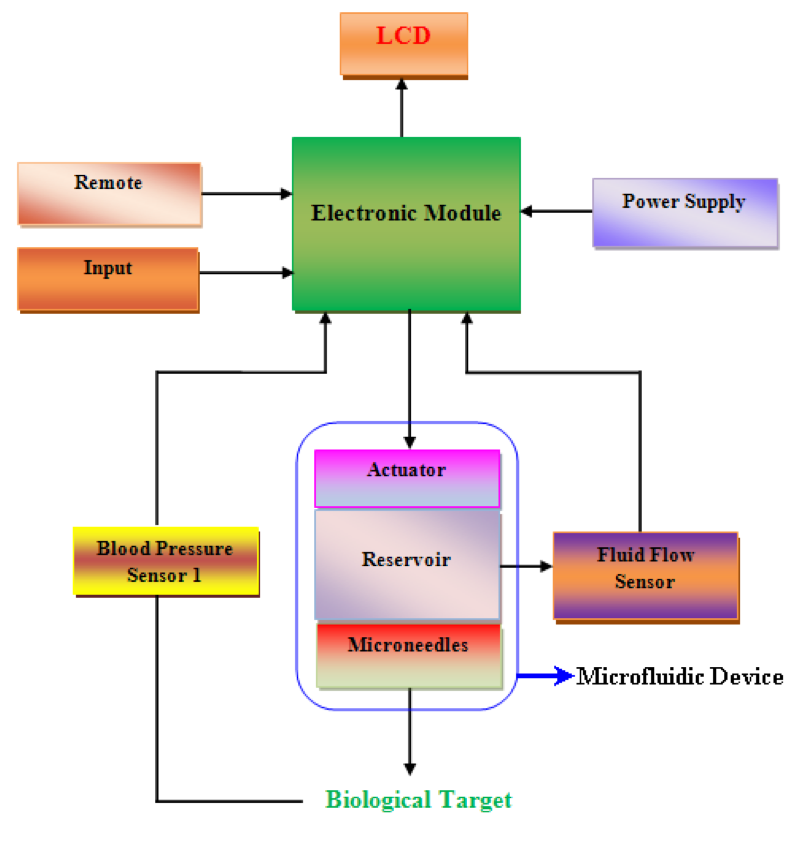
\includegraphics[width=\linewidth]{Chapter2/Figs/Raster/TDD.png}
    \caption{Diagram of transdermal drug delivery system that shows interaction of electronic system with a power suppy, and a microfluidic device corresponding to an actuator, a reservoir, and microneedles.}\label{tdd}
\end{figure}

In both the scenario in which one wishes to directly characterize the mechanical properties of cells in their natural environments, and in which one wants to construct immersed actuators for micro-fluidic systems, an electrostatic actuator that can be effectively operated in electrolytes is of critical importance.

\section{Electrostatic Comb-Drives and In Vivo Cell Characterization}
As detailed in the previous section, electrostatic comb-drive actuation in electrolytes will enable the study of cells under conditions that mimic their natural conditions. In this section, we will detail experiments that demonstrated the feasibility of using electrostatic comb-drive actuators to measure the stiffness of cells in their natural conditions. Before doing so, we review the difficulties of operating electrostatic actuators in electrolytic media, and the manner in which these difficulties were overcome. 

The behavior of the comb-drive actuator is traditionally understood by abstracting away its geometry. A common method for modeling the comb-drive is to view the overlapping components of the interdigitated fingers as a pair of parallel plates, figure \ref{finger_to_plates}. When DC voltages are applied to a comb-drive actuator in air, the potential profile between them is linear, resulting in an attractive force between the fingers. In an electrolyte, however, ions collect on the fingers and form the Stern layer and electric double layer (EDL). These layers prevent a potential drop between the fingers, thus preventing displacement in a process called ionic shielding, figure \ref{pot_profiles}. Sounart et al. discovered that this issue could be overcome by applying AC signals at frequencies faster than the time necessary for ionic shielding\cite{Sounart2005}. 

\begin{figure}[h]
    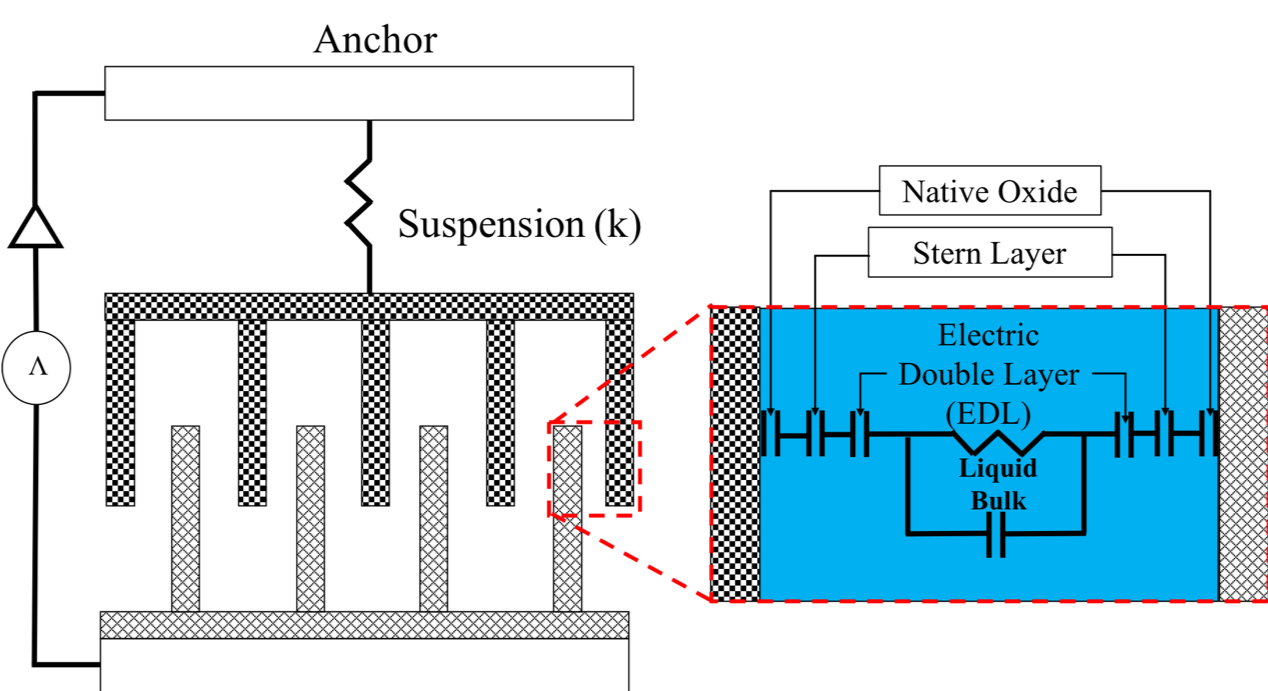
\includegraphics[width=\linewidth]{Chapter2/Figs/Raster/fingers_to_plates_electrolyte.png}
    \caption{Schematic of a comb-drive actuator, and the model of its overlapping fingers when the actuator is immersed in an electrolyte. When a voltage is applied between the inter-digitated fingers, the fingers attached to the spring move parallel to the  stationary fingers. The moving structure is grounded so that no capacitance is formed between the comb-drive and the substrate.} \label{finger_to_plates}
\end{figure}

\begin{figure}[h]
    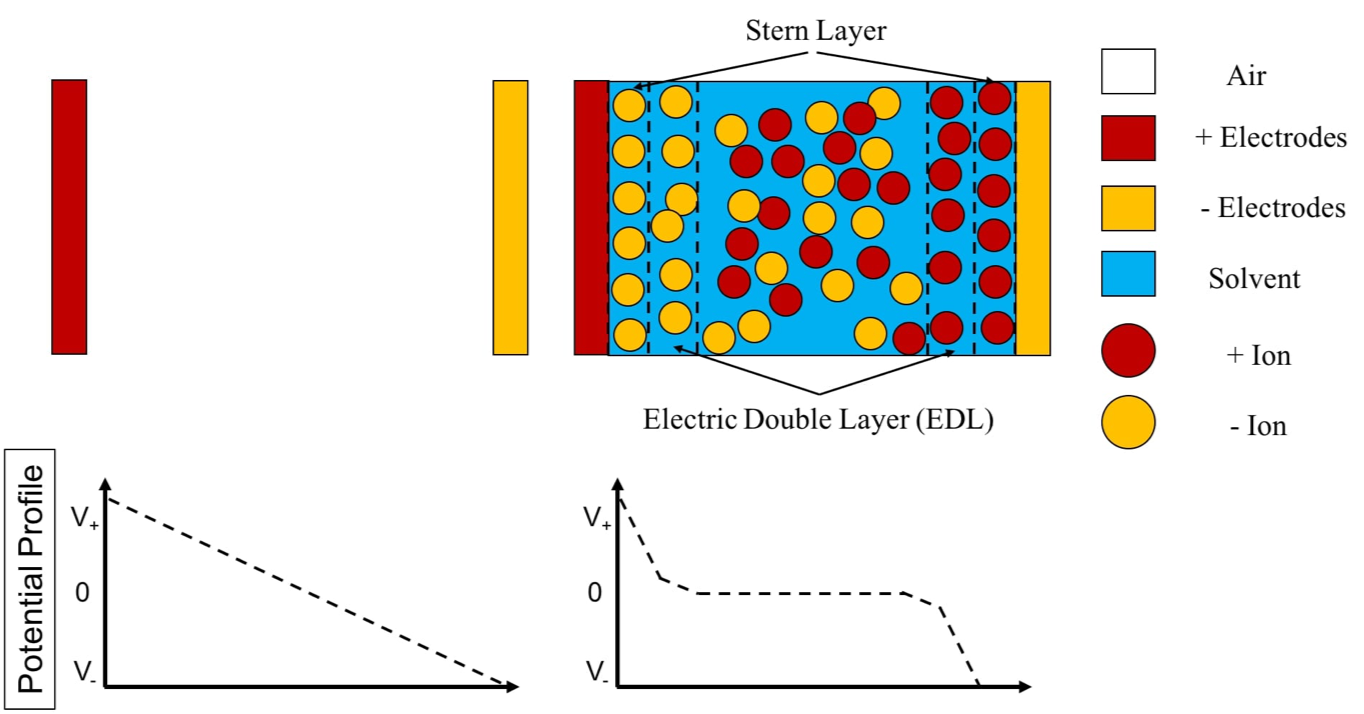
\includegraphics[width=\linewidth]{Chapter2/Figs/Raster/potprofile_air_vs_electrolyte.png}
    \caption{Pair of fingers in air (left), and electrolytes (right) under DC voltage along with their potential profiles as a function of distance between the fingers. The potential profile in air is linear, while the profile in the electrolyte is flat in the bulk, because of the voltage drop in the EDL and Stern layers.} \label{pot_profiles}
\end{figure}

\begin{figure}[htpb]
    \begin{center}
    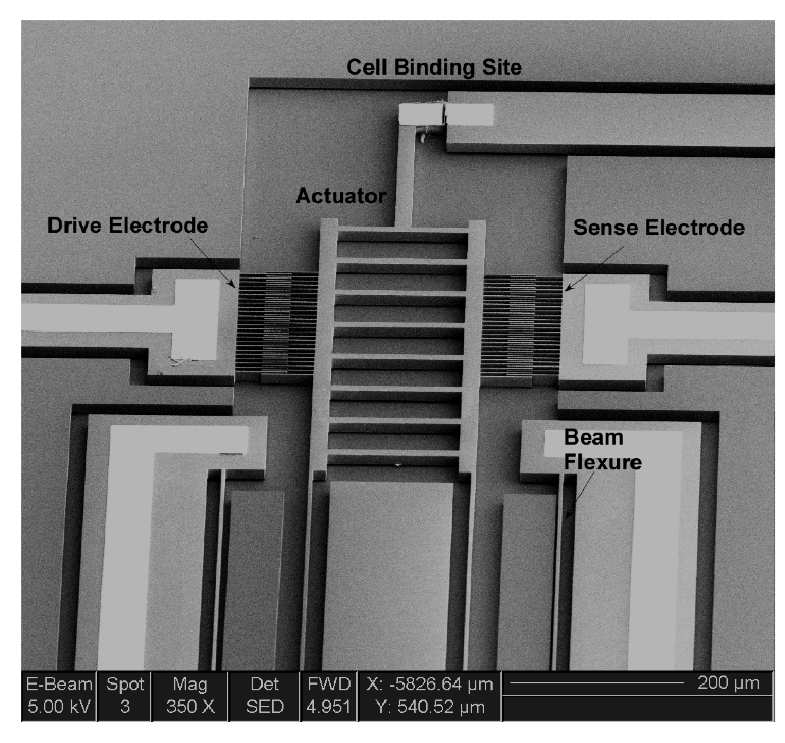
\includegraphics[width=0.6\linewidth]{Chapter2/Figs/Raster/vikramDesgn1.png}
    \caption{Image of Mukundan et al.'s first design of the comb-drive actuator to be immersed in an electrolyte.} \label{vik_design_1}
    \end{center}
\end{figure}

\begin{figure}[htpb]
    \begin{center}
    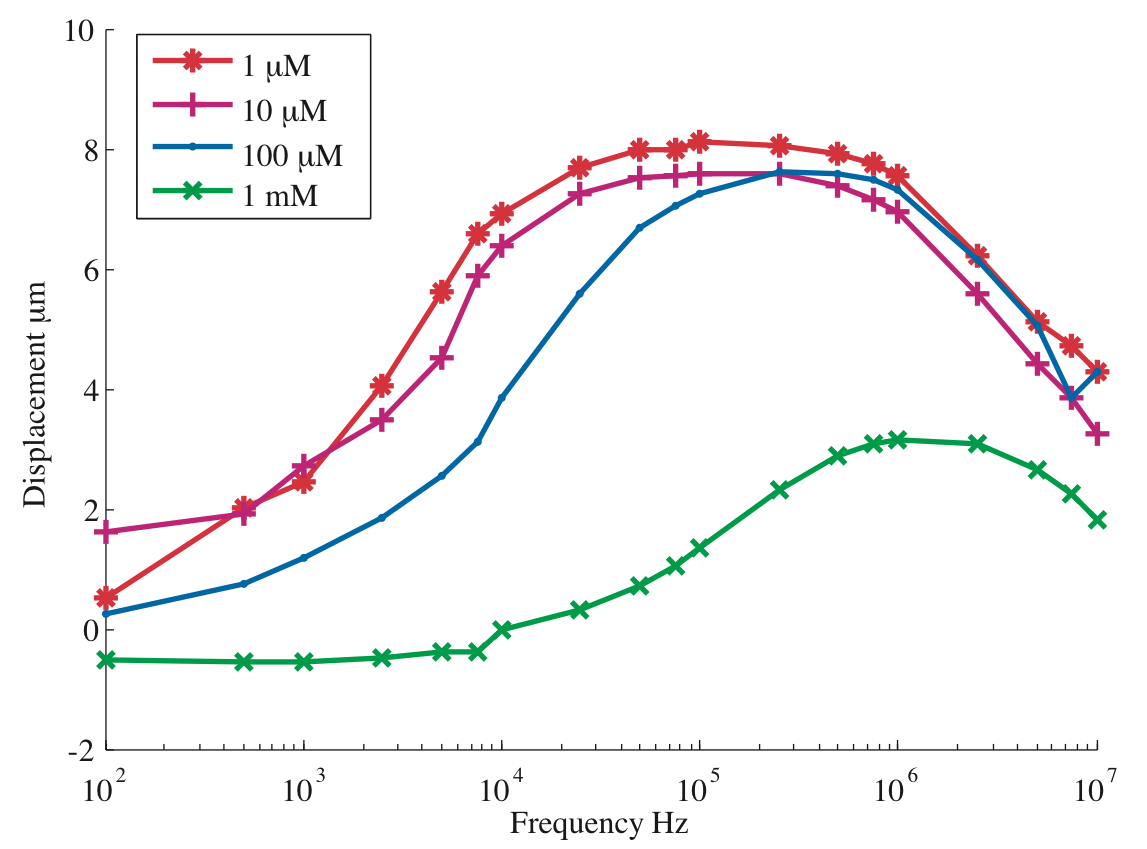
\includegraphics[width=0.6\linewidth]{Chapter2/Figs/Raster/displacementAttenuationDesgn1.png}
    \caption{Plot of displacement of the comb-drive actuator in electrolytes for Mukundan et al.'s first actuator design, as a function of frequency. The displacement decreases as frequency increases, a clear sign of parasitic impedance} \label{disp_attenuation}
    \end{center}
\end{figure}
The principle discovered by Sournat et al. were used in subsequent work by a variety of author's, in particular Mukundan et al, and Panchawagh et al \cite{Mukundan2009,MukundanandPonce2009,Panchawagh2009}. The goal of Mukundan et al.'s work was to use the comb-drive actuator in biological media, so that they could demonstrate the feasibility of using this device to actuate biological cells. The frequencies required to overcome shielding effects in biological media is minimally about one MHz. This frequency corresponds to the level at which the parasitic impedance of typical MEMs devices begins to impact their designed behavior. The originally designed device corresponds to a single flat-head tip, fabricated next to a fixed structure \cite{Mukundan2009}. This flat-head tip and fixed structure is the location to which cells were intended to bind. The flat-head tip is attached to an actuator structure. A drive comb-drive is connected to one side of the structure, and a sensor comb-drive is connected to the other, figure \ref{vik_design_1}. The end of the actuator structure furthest from the flat-head tip was attached to a folded-flexure, which facilitated its motion. When this device is operated in biological media, the distortion of the signal due to parasitic impedance results in decreasing displacement as frequencies increase above 1 MHz, figure \ref{disp_attenuation} \cite{Mukundan2009}. 

In order to overcome this, Mukundan et al. introduced what they termed a differential design, figure \ref{vik_design_2} \cite{Mukundan2009}. This structure was composed of a pair of adjacent flat-head tips, one for actuation and the other for sensing. The actuation flat-head was attached to an actuator structure with an equal number of drive comb-drives on each side. In this scenario, AC signals of opposite polarity were applied to the set of drive electrodes on each side. This resulted in approximately zero net current to the device substrate, and minimized the impact of parasitic impedance on the comb-drive actuators operation at high frequencies in biological media \cite{Mukundan2009}, figure \ref{disp_attenuation} 

\begin{figure}[htpb]
    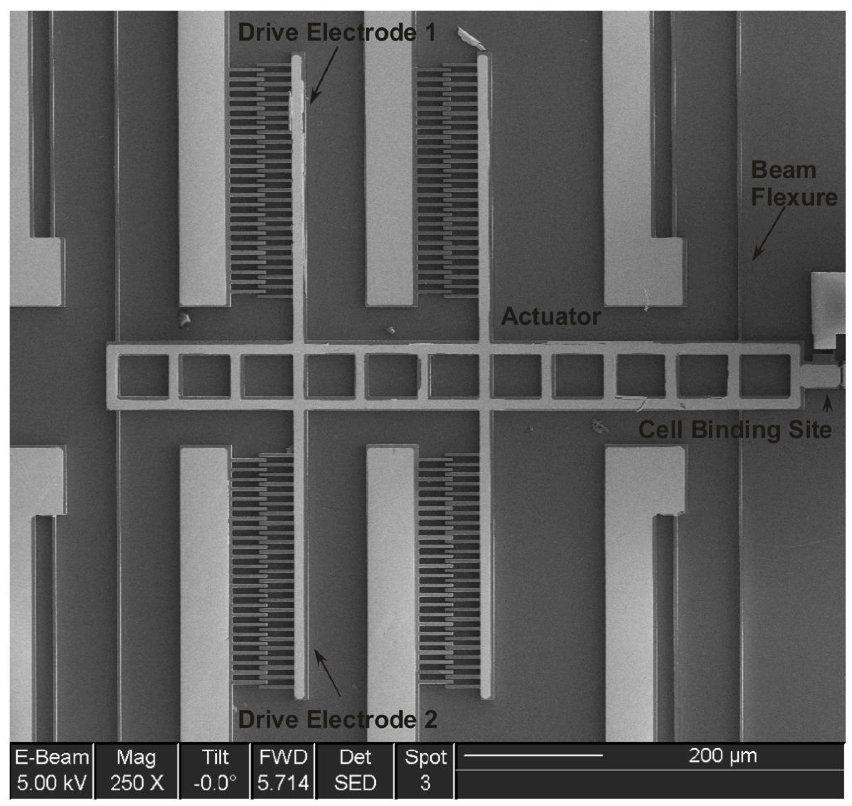
\includegraphics[width=\linewidth]{Chapter2/Figs/Raster/vikramDesgn2.png}
    \caption{Image of Mukundan et al.'s second comb-drive actuator design, which combats the issue of attenuation when actuated at high frequencies, and immersed in electrolytes} \label{vik_design_2}
\end{figure}

\begin{figure}[htpb]
    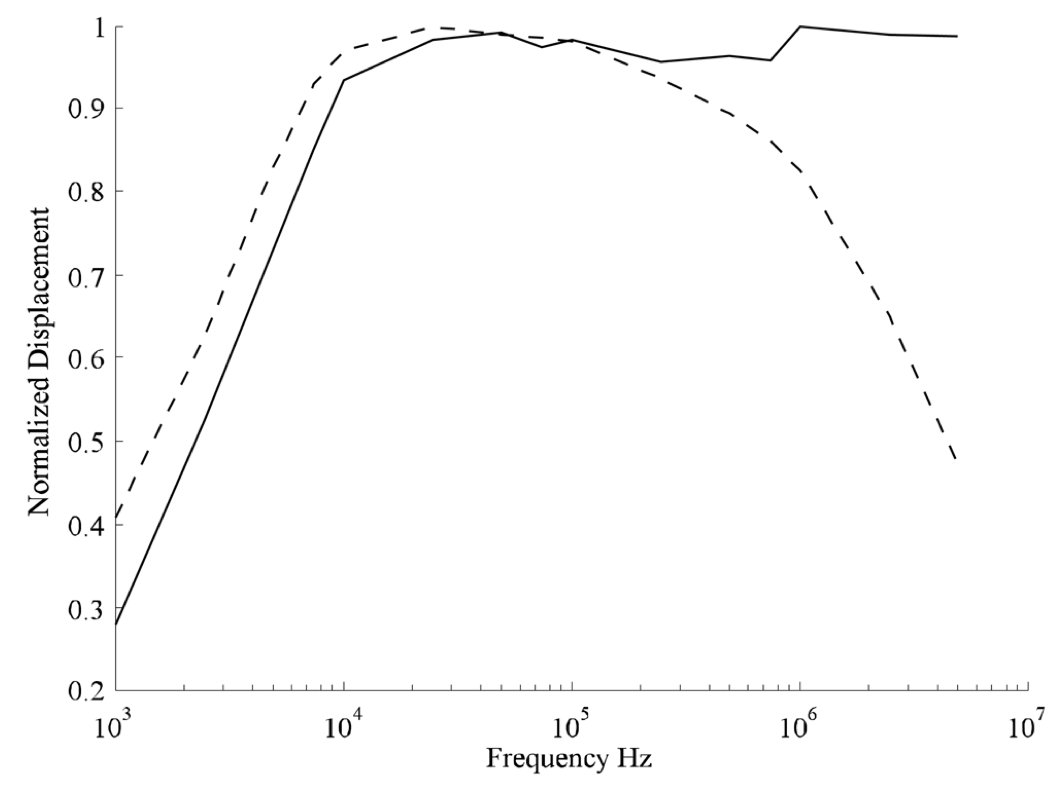
\includegraphics[width=\linewidth]{Chapter2/Figs/Raster/displacementAttenuationDesgn2.png}
    \caption{Plot of displacement of the comb-drive actuator in electrolytes for Mukundan et al.'s second actuator design, as a function of frequency. The displacement does not attenuate as severely as in the first design.} \label{vik_design_2}
\end{figure}

The final difficulty in operating comb-drive actuators in biological media is electrolysis. If AC signals of frequencies below a certain threshold are applied to the comb-drive, then electrolysis will occur at the comb-drive fingers, corroding the fingers and releasing air bubbles within the device. This threshold frequency increases as with increasing concentration. Mukundan et al. found that this could be avoided above 10 KHz for media with electrolyte concentrations at, or above, 10mM \cite{Mukundan2009}.

To the author's knowledge, the first demonstration of using a submerged electrostatic comb-drive actuator to mechanically test cells is was done by Mukundan et al. in 2009\cite{Mukundan2009}. The differential design device described earlier in this section was used to stretch Madine-Darby Canine Kidney (MDCK) cells. The flat-head tips were patterned with gold, so that the cells would adhere to them. In order to precisely place the MDCK cells on these flat-head tips, the authors used a micropipette and micromanipulator. This prevented cells from spreading through out the device, and impeding it's performance. It is important to note that the sensor flat-head tip was essentially fixed during their experiments, and that the displacement of the actuator flat-head is measured optically. The stiffness of the comb-drive device, and of the cell sample, is found by comparing the displacement and square-voltage curves of the actuating flat-head, both with and without a cell. The cell stiffness was then used to estimate the force it experienced, figure \ref{fab_steps}.

\section{Device Fabrication}
In this section, we describe how the device is fabricated, and how it is prepared for experiments. The devices were fabricated as in Mukundan et al. Specifically, they were created on silicon-on-insulator (SOI) wafers with a 15 $\micro$m device layer. The relevant features were initially patterned in the silicon through a deep reactive ion etch (DRIE) process, and E-beam evaporation was used to deposit a composite metal layer that is made of chromium (Cr 25 nm)/platinum(Pt 50 nm)/gold(Au 300 nm). Gold was used because it resists corrosion under AC voltages in electrolytes, and is bio-compatible. Finally, parylene-C was used as passivation for the electrodes. The steps in the process are shown in figure \ref{fab_steps}. 

\begin{figure}[htpb]
    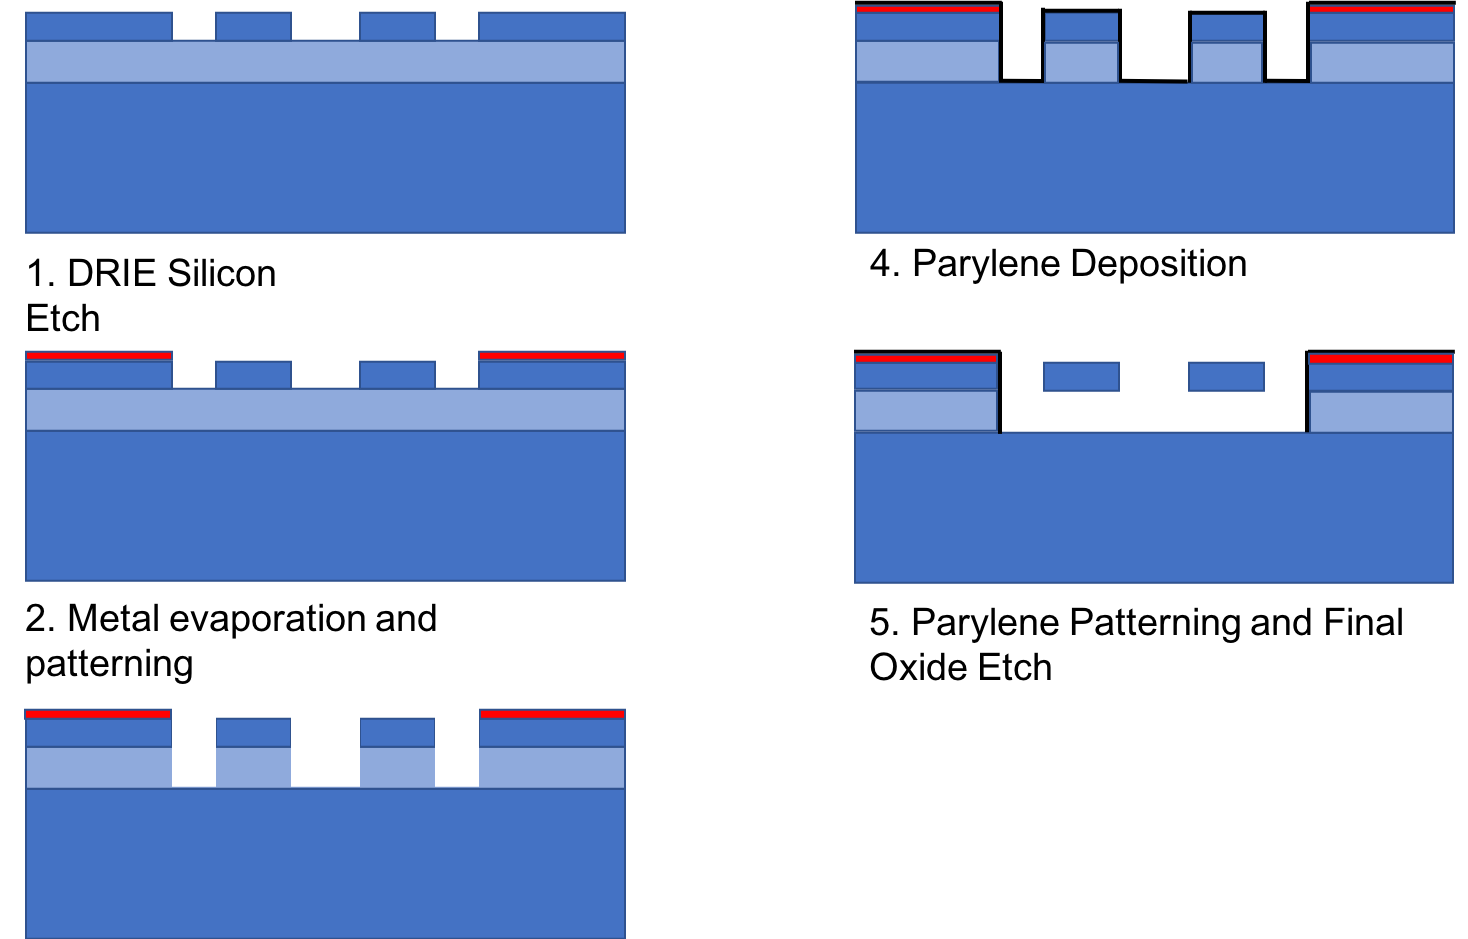
\includegraphics[width=\linewidth]{Chapter2/Figs/Raster/fabricationStepsDesgn2.png}
    \caption{Pictorial representation of sequence of fabrication steps used to create the comb-drive actuator used in this thesis, figure \ref{vik_design_2}}\label{fab_steps}
\end{figure}

\begin{algorithm}[H]
\caption{Preparing Device for Experiments}\label{euclid}
\begin{algorithmic}[1]
%\Procedure {}
\State  Micro-pipette an alcoholic solution onto the device in the DIP
\State (Optional) Immerse the entire DIP in a petri-dish of alcoholic solution, wrap it inpara-film, and allow to sit for 12-24 hours
\State $i = 0$
\While{$i \leq 8$}
    \State Micro-pipette a small amount of the alcohol out of the DIP
    \State  Micro-pipette a small amount of the aqueous solution into the DIP
    \State $i \leftarrow i+1$
\EndWhile
\State When ready to store, leave the DIP in a petri-dish of alcoholic solution, or aqueous solution and seal it with para-film.
\State \textbf{Note 1:} When replacing aqueous solution with a larger concentration of electrolytes with one with a smaller concentration, first replace the aqueous solution with alcohol, and then replace the alcohol with the new aqueous solution. The process of replacing liquids is as described in 3-5.
\State \textbf{Note 2:} Dry the device with a Critical Point Drier. If the device is allowed to dry in air, droplets will develop and damage the structure. 
%\EndProcedure
\end{algorithmic}
\end{algorithm}

\section{Preparing Device for Experiments}
The treatment of the devices post-fabrication is critical to it's successful use in experiments. The devices were mounted on ceramic dual in-line packages (DIP) using quick setting epoxy, after which the devices were allowed to sit for 12-24 hours. Gold wire-bond were then used to attach the pads on the device to the relevant pads on the DIP. Gold wire was used because it does not react with electrolytic liquids when subjected to sufficiently high frequency AC signals. The pads that correspond to the actuator structure are connected to ground, while the fixed comb-drives on either side of the actuator structure are attached to pins on the DIPs that take AC signals of opposite polarities as inputs. 

Before the device can be immersed in electrolytic liquids, it is necessary to wet it with an alcoholic solution first (at least ninety percent alcoholic), like isopropanol. If the device is immediately exposed to an electrolytic liquid, the surface tension of the aqueous solution will lead to the formation of drops that crush structures in the device, and cause irreparable deformation to the folded-flexures attached to the actuator structure. Wetting the device with alcohol first prevents the formation of drops when it is immersed in an aqueous solution. The steps of wetting are given by algorithm 1, figure \ref{wet_steps}. 

\begin{figure}[htpb]
    \begin{center}
    \includegraphics[width=0.3\linewidth]{Chapter2/Figs/Raster/placeholder.png}
    \caption{Placeholder for image of wetting steps}\label{wet_steps}
    \end{center}
\end{figure}


\begin{comment}
\begin{enumerate}
    \item Micro-pipette an alcoholic solution onto the device in the DIP 
    \item (Optional) Immerse the entire DIP in a petri-dish of alcoholic solution, wrap it in para-film, and allow to sit for 12-24 hours.
    \item Micro-pipette a small amount of the alcohol from the DIP
    \item Micro-pipette a small amount of the aqueous solution into the DIP
    \item Repeat steps 3 and 4 until all the liquid in the DIP is the aqueous solution
    \item When ready to store, leave the DIP in a petri-dish of alcoholic solution, or aqueous solution and seal it with para-film
    \item \textbf{Note 1:} When replacing aqueous solution with a larger concentration of electrolytes with one with a smaller concentration, first replace the aqueous solution with alcohol, and then replace the alcohol with the new aqueous solution. The process of replacing liquids is as described in 3-5.
    \item \textbf{Note 2:} Dry the device with a Critical Point Drier. If the device is allowed to dry in air, droplets will develop and damage the structure. 
\end{enumerate}
\end{comment}



\section{Experimental Pipeline}
In this section we describe the semi-automated experimental pipeline that was designed and built to collect data. We first discuss the software and hardware necessary for this pipeline. We subsequently describe how we prepare for a particular experiment, the process of running experiments, and the method by which we post-process collected data. The code associated with this is located on github, and is copied in the appendix \cite{Dibua2018DataCollect}. \textbf{Appendix}

\subsection{Software and Hardware Requirements}
The software requirements of our experimental pipeline are,

\begin{itemize}
    \item Python 2.7 or greater
    \item OpenCV (Python)
    \item Matlab
    \item GPIB Matlab
    \item Micromanager 
\end{itemize}

while the hardware requirements are

\begin{itemize}
    \item Leica Upright Microscope $\times$1
    \item TEK AFG 3102a Function Generator $\times$1
\end{itemize}

\subsection{Running an Experiment}
\subsubsection{Mounting the Device}
The process of running an experiment starts with mounting the device on the microscope, and connecting it to the function generator for the purpose of actuation. The device is submerged in an aqueous solution, following the steps described in section 2.5. This device is then placed on a chip-holder, which has been soldered to a PCB. The PCB is wired such that pins one and twenty-four are grounded, while pins three to six and nineteen to twenty-two are connected to different channels of the function generator, which applies signals that ninety degrees out of phase with each other. This PCB should already have been connected to the channels of the function generator. Figure \ref{empty_mount}, shows the chip-holder with all of the relevant connections, and figure \textbf{Image of PCB with Chip} shows DIP with the PCB.

\begin{figure}[htpb]
    \begin{center}
    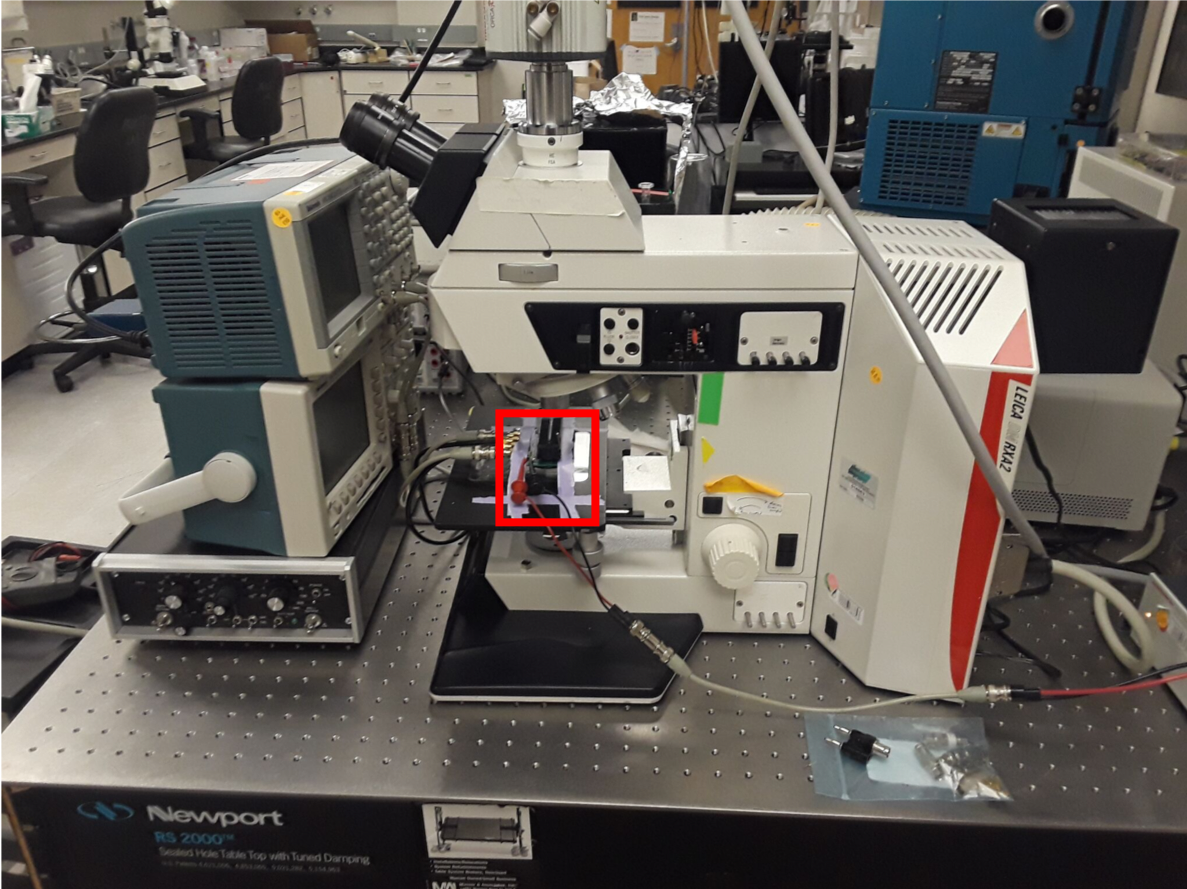
\includegraphics[width=0.8\linewidth]{Chapter2/Figs/Raster/pcb_no_dip.png}
    \caption{Image of the chip-holder on which the DIP will be mounted. The chip-holder is attached to a function generator and oscilloscope, and the tape is used to keep it flat while the microscope is moved in order to focus the image. The chip holder is bounded by a red box.}\label{empty_mount}
    \end{center}
\end{figure}

\begin{figure}[htpb]
    \begin{center}
    \includegraphics[width=0.5\linewidth]{Chapter2/Figs/Raster/placeholder.png}
    \caption{Placeholder for image that will show pcb mounted on a DIP}\label{pcb}
    \end{center}
\end{figure}

\begin{figure}[htpb]
    \begin{center}
    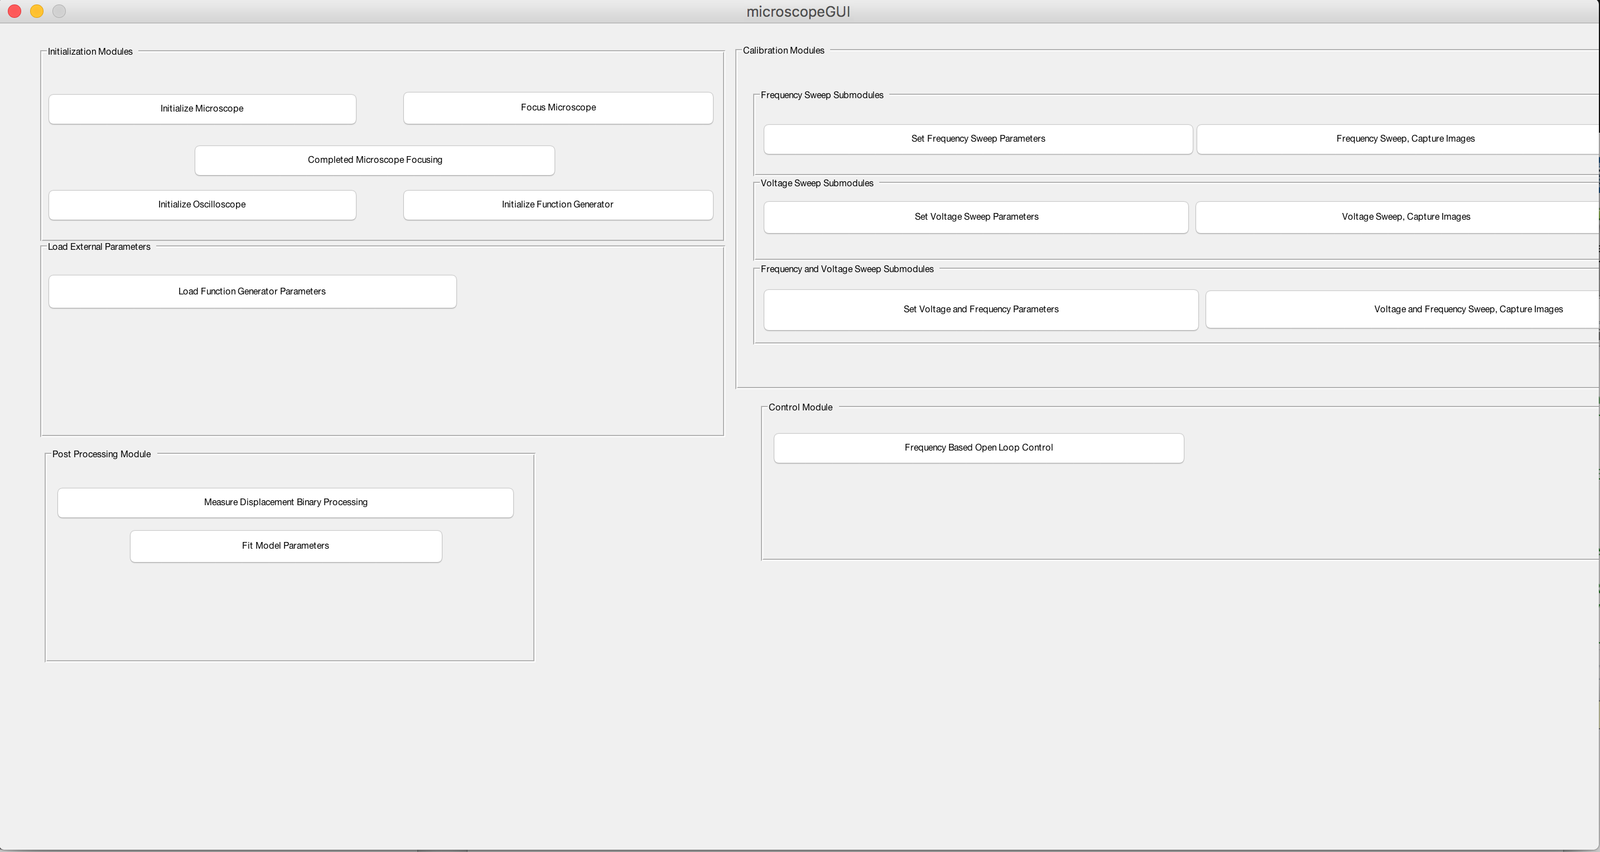
\includegraphics[width=0.9\linewidth]{Chapter2/Figs/Raster/guioptions.png}
    \caption{Options that appear when the MATLAB GUI that facilitates the semiautomatic collection of experimental data is initialized.}\label{gui_options}
    \end{center}
\end{figure}
\subsubsection{Initializing the Semi-auomated Data Collection Software}
After mounting the device, the Matlab GUI is turned on, and the microscope, function generator, and digital oscilloscope are initialized with button clicks in that order. Upon initializing the microscope, the user is asked to move the Microscope stage to a maximum and minimum height. This is will act as the bounds of the stages motion when it is moved during the process of auto-focus, and will prevent the device from crashing into the microscope lens. After this, an image of the device under the lens pops up, and the user is expected to focus the image, and click, "Complete Focus" in the GUI, after they are satisfied. 



The final aspect of initialization involves defining parameters for the experiment to be run. Clicking the Frequency sweep button will allow the user to set the maximum and minimum log of the frequency to be used in the experiment, the number of points in that range (log-spaced), the voltage of the applied signal, the number of trials to be run for these setting, and the interval of trials needed before the user is given a chance to manually focus the image, figure \ref{gui_options}. 



\subsubsection{Addressing the Challenges of Semi-automated Data Collection}
After initializing the software, the click of a button will begin the process of data collection. The channels of the function generator are set to the prescribed voltage amplitude, initialized to the proper frequency, and made 90 degrees out of phase before being turned on. Algorithm 2 outlines the manner in which the semi-automated data collection proceeds. In the algorithm, $n_{trials}$ is the number of trials chosen by the user for a particular experiment, $n_{frequency}$ the number of points selected in log space between a minimum and maximum frequency, and $n_{interval}$ is the interval of trials the user selects between which the automated data collection pauses. 


For the purpose of clarification, we will expand on some of the steps of the semi-automated data collection process. In particular, we expand upon line 16, the auto-focusing of the image, and lines 20-24, pausing data collection pending user input. During the process of running our experiments, the aqueous solution slowly evaporates. This leads to two issues. The first is that the image focus grows worse over time. The second is that the device can become dry in air, leading to damage to the comb-drive structure. 
\begin{algorithm}[H]
\caption{Semi-automated Data Collection}\label{euclid}
\begin{algorithmic}[1]
%\Procedure {}
\State Turn function generator channels off
\State Initialize function generator to $v_{init}$
\State Take and save image of device before motion
\State Initialize array of images, $I$
\State $i \leftarrow 1$
\While{$i \leq n_{trials}$}
    \If {$i=1$}
        \State Pause process pending user input
        \State Add aqueous solution to device to keep it wet
        \State Manually focus image if necessary 
        \State Turn on channels of function generator
    \EndIf
    \State $k \leftarrow 1$
    \While{$k \leq n_{frequency}$}
        \State Set function generator to the $kth$ frequency
        \State Automatically focus the image
        \State Take picture of device, and store in $I$
        \State $k \leftarrow k+1$
    \EndWhile
    \If {$rem(i,n_{interval})=0$}
        \State Pause process pending user input
        \State Add aqueous solution to device to keep it wet
        \State Manually focus image if necessary 
    \EndIf
    \State Save stored images to file
    \State $i \leftarrow i+1$
\EndWhile
%\EndProcedure
\end{algorithmic}
\end{algorithm}

\begin{algorithm}[H]
\caption{Golden-Section Search: Autofocus using GLLV}\label{euclid}
\begin{algorithmic}[1]
%\Procedure {}
\State Initialize $x_{l}*$ and $x_{u}*$
\State Initialize $x_l$ and $x_u$
\State Initialize $n_{max}$
\State Initialize $tol$
\State $k \leftarrow 1$
\While{$k<=n_{max} \text{ or } |x_l-x_u|>tol$}
    \If {$k=1$}
        \State $d = \frac{(\sqrt{5}-1)}{2}(x_u-x_l)$
        \State $x_1 = x_l + d$
        \State $x_2 = x_u - d$
    \EndIf
    \If {$x_1 < x_{u}* \text{ and } x_2 > x_{l}*$}
        \If {$f(x_1) > f(x_2)$}
            \State $x_l \leftarrow x_2$
            \State $x_2 \leftarrow x_1$
            \State $d = \frac{(\sqrt{5}-1)}{2}(x_u-x_l)$
            \State $x_1 = x_l + d$
        \Else 
            \State $x_u \leftarrow x_1$
            \State $x_1 \leftarrow x_2$
            \State $d = \frac{(\sqrt{5}-1)}{2}(x_u-x_l)$
            \State $x_2 = x_u - d$
        \EndIf
        \State $k \leftarrow k+1$
    \Else
        \State End While
    \EndIf
\EndWhile
%\EndProcedure
\end{algorithmic}
\end{algorithm}

We addressed the first issue by developing an auto-focusing algorithm. An auto-focusing algorithm has two main components. The first is defining a measure of focus that is useful for a particular application, and the second is implementing an optimization algorithm for maximizing, or minimizing, this measure. Pertuz et al. reviewed a variety of focus measures that were introduced in literature over the past two decades\cite{Pertuz2013}. Of these measures, we found that the Graylevel Local Variance (GLLV) worked well with our application. The GLLV essentially calculates the variance of the gray-levels of an image in neighborhoods of an image, and is expressed as

\begin{equation}
    \phi_{x,y} = \sum_{(i,j) \in \Omega(i,j)(x,y)} (L_{v}(i,j) - \overline{L}_v)^2,
\end{equation}

where $\phi$ is the measure, $L_{v}(i,j)$ is the variance of the gray-level in a neighborhood $w_x \times w_y$, and $\overline{L}_v$ is the mean of the gray-level in that area. This measure is maximized using the golden-section search method.

The golden-section search optimization method is constructed to find the minimum or maximum of a univariate function that is unimodal over the interval of optimization\cite{Nazareth2002}. The input to the golden-section algorithm, when optimizing the GLLV, is the height of the microscope stage. As long as the height at which the image can be focused is contained in the interval of heights being searched, the GLLV satisfies the unimodal assumption. Our implementation of the golden-section method is described in algorithm 3. In this implementation of the golden-section search, $x_l$ and $x_u$ are the minimum and maximum heights in the interval to be searched, $n_{max}$ is the maximum number of iterations of this algorithm, and $tol$ is the distance between $x_u$ and $x_l$ at which the optimization stops. Finally $x_{l}*$ and $x_{u}*$ are minimum and upper heights defined for the purposes of protecting the microscope lens. The microscope stage is should not move beyond these bounds if the optimization is properly implemented. Figure \ref{golden_section_pic} represents this algorithm pictorially.

\begin{figure}[htpb]
    \begin{center}
    
\includegraphics[width=0.6\linewidth]{Chapter2/Figs/Raster/golden_section_figure.png}
    \caption{Example of function being optimized by one step of the golden-section algorithm.}\label{golden_section_pic}
    \end{center}
\end{figure}

The second issue was addressed more simply. Rather than automating the entire experiment, we allowed the code to pause the data collection every $n$ trials, so that the user can keep the device wet.

\subsection{Post-Processing the Collected Data}
This section focuses on how the collected data is post-processed. It describes the standard method for measuring the displacement of the device pads, and the problems with robustness that this method faces. Finally, it details a new, and more robust, method for calculating the device pad displacement. We will show the impact of the different processing steps on two pads in our device when viewed using a 50x air microscope, figure \ref{orig_device}.

\begin{figure}[htpb]
    \begin{center}
    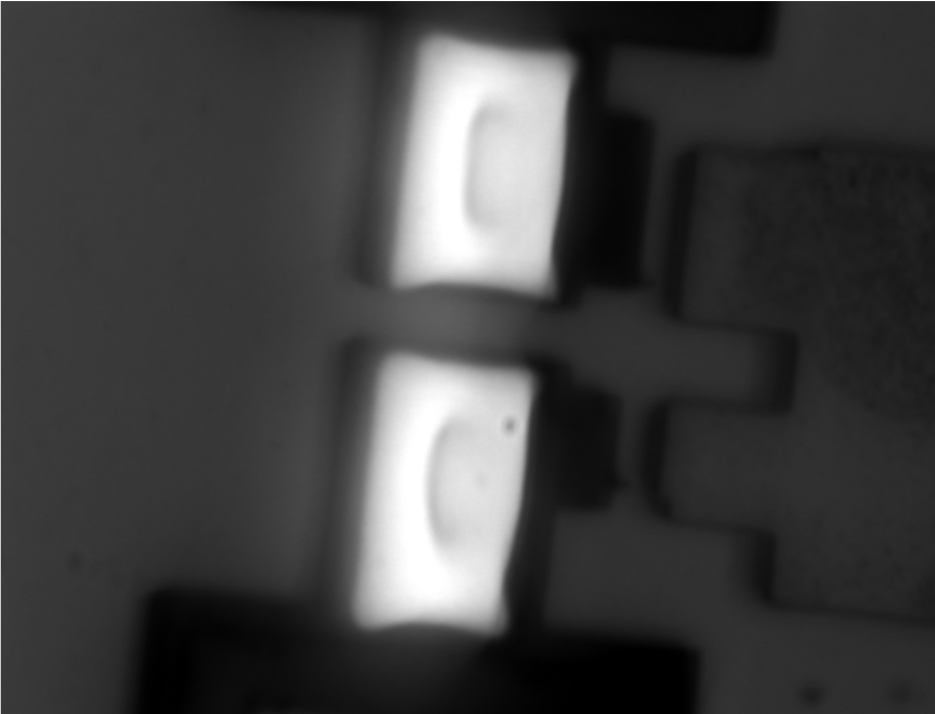
\includegraphics[width=0.6\linewidth]{Chapter2/Figs/Raster/device_processed_displace.png}
    \caption{Image of two pads of the comb-drive viewed under 50x air microscope, before any user processing.}\label{orig_device}
    \end{center}
\end{figure}

\subsubsection{Standard Method for Measuring Displacement}
The first step in measuring the displacement of the pads was transforming the image from gray-scale to binary, using a global threshold value for gray-scale intensity,$i_{th}$. This results in an image with potential holes in the contours. These holes are filled, resulting in an image with two contours corresponding to the device pads, figure \ref{binary_contour}. The device pads are then found using the area of these contours. Finally, the centroids of the contours corresponding to the pads are calculated. The change in distance between these centroids from image to image is the displacement.

This process, while promising, is not robust. In particular, this method of processing the data is sensitive to the threshold value for gray-scale intensity, $i_{th}$. Slightly different values of gray-scale intensity results in large variations of the discovered contours, and, by extension, the calculated displacement, as well as in the variance of these measurements. Figure \ref{binary_meas} shows the noisy measurements of what should be a relatively smooth pad motion, based on this processing method.
The source of this sensitivity is the change in lighting of the device that occurs over the course of an experiment. The two main sources of this change in lighting are the actuator device pad motion, and the evaporation of the aqueous solution. 

In order to credibly validate a set of models, it is critical that the data is post-processed in the most robust manner possible.

\begin{figure}
    \centering
    \begin{minipage}{0.48\textwidth}
        \centering
        
\includegraphics[width=\textwidth]{Chapter2/Figs/Raster/binary_contours.png} % first figure itself
        \caption{Binary contours found when using the standard method for measuring displacement.}\label{binary_contour}
    \end{minipage}\hfill
    \begin{minipage}{0.48\textwidth}
        \centering
        
\includegraphics[width=\textwidth]{Chapter2/Figs/Raster/adaptive_contours.png} % second figure itself
        \caption{Binary contours found when using localized measure of displacement method for measuring displacement.}\label{adaptive_contour}
    \end{minipage}
\end{figure}

\subsubsection{Localized Method for Measuring Displacement}
Before discussing our alternative pipeline for measuring displacement, we briefly discuss adaptive local thresholding. Adaptive local thresholding is a method of making images binary that combats variations in illumination within, and across, images. It uses the grayscale valus of a small neighborhood, $w_x \times w_y$, around $(x,y)$ in order to determine whether or not a pixel is background or foreground. In particular,

\begin{equation}
    p(x,y) = 
        \begin{cases}
         m      & \text{if } p_0(x,y) > T(x,y) \\
         0       &   \text{otherwise} 
         \end{cases}
\end{equation}

where $p(x,y)$ is the value of pixel $(x,y)$ in the binary image, $p_0(x,y)$ is the intensity of pixel $(x,y)$ in the gray-scale image, and $T(x,y)$ is the mean gray-scale intensity of the pixels in the neighborhood of size $w_x \times w_y$ centered on $(x,y)$, sometimes subtracted from some prescribed value $c$. This particular technique is called the adaptive threshold method. It works best under the conditions in which an image contains a comparable amount of background and foreground\cite{GW2008}. When this is not the case, neighborhoods contain only foreground, or background, making this method ineffective. 

Our alternative pipeline begins by binarizing our images using local thresholding. The resulting contours are further filtered using two criteria. The first criteria are bounds on the areas of the contours, similar to the standard method for measuring displacement. The second is that the only valid contours are those that are approximately rectangles. The rest of the processing pipeline proceeds as in the standard method. The contours that results from this process closely replicate the shape of the pads in the original image and are consistent across an experiment, without needing to tune any parameters, figure \ref{adaptive_contour}, as well as yield robust measurements of displacement, figure \ref{adaptive_meas}.

\begin{figure}
    \centering
    \begin{minipage}{0.48\textwidth}
        \centering
        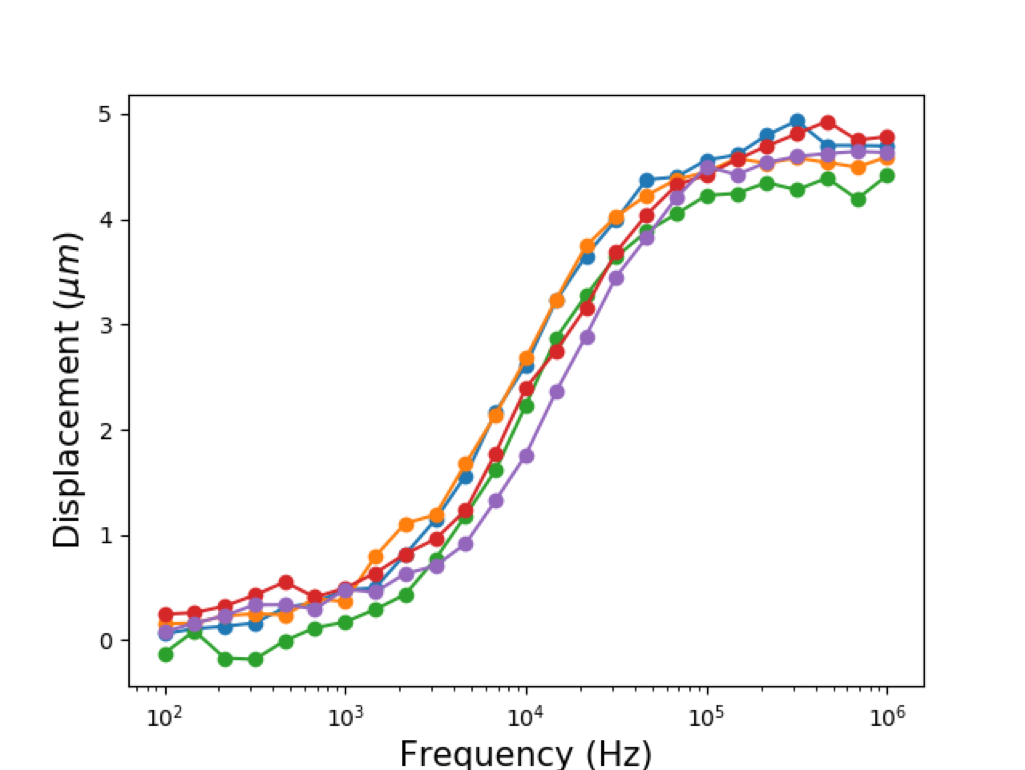
\includegraphics[width=1.1\textwidth]{Chapter2/Figs/Raster/disp_binary.png} % first figure itself
        \caption{Five trials of measured displacement of actuator pads using standard methods for measuring displacement as a function of frequency when actuated by a 4 $V_{p-p}$ signal.}\label{binary_meas}
    \end{minipage}\hfill
    \begin{minipage}{0.48\textwidth}
        \centering
        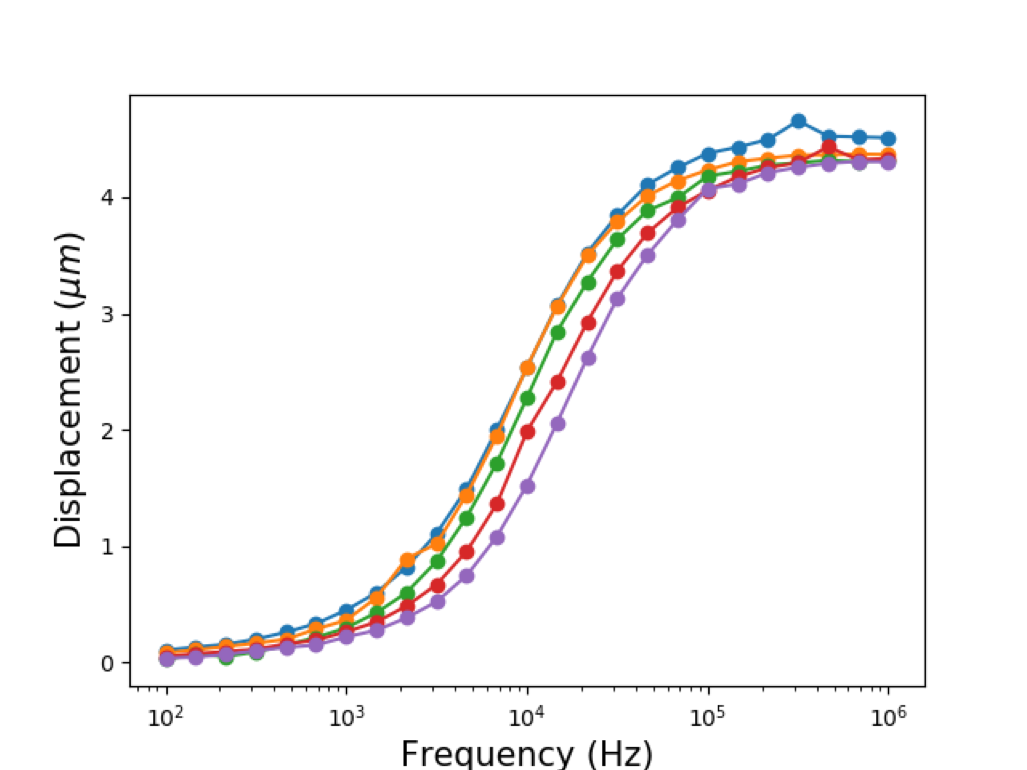
\includegraphics[width=1.1\textwidth]{Chapter2/Figs/Raster/disp_adaptive.png} % second figure itself
        \caption{Five trials of measured displacement of actuator pads using local method for measuring displacement as a function of frequency when actuated by a 4 $V_{p-p}$ signal.} \label{adaptive_meas}
    \end{minipage}
\end{figure}

\section{Experimental Conditions for Data Collection}
We have detailed the construction of a semi-automated pipeline for measuring the displacement of a comb-drive actuator in electrolytes. In this section, we detail the conditions under which we measure comb-drive displacement. We collect data at 0.1 $mM$, 0.5 $mM$, 1 $mM$, and 10 $mM$ KCl. At each concentration, we perform five trials of frequency sweeps, and, in each trial, 25 log-spaced frequencies are selected for actuation. The range of frequencies swept is from 100 $Hz$ to 1 $MHz$ at concentrations of 0.1 $mM$, 0.5 $mM$, and 1 $mM$ KCl, and between 1 $KHz$ to 10 $MHz$ for a concentration of 10 $mM$. We collect data for the described conditions for two types of comb-drive. One is a comb-drive with 200 pairs of fingers separated by a gap of 2 $\mu m$, and the second is one with 100 pairs of fingers separated by a gap of 5 $\mu m$. Unless otherwise stated, the data used for validating models will be pulled from the above described set of experiments. 
\section{Chapter Review and Further Work}
In this chapter, we gave a brief background on the use of MEMS devices to mechanically characterize cells, discussed the potential utility of electrostatic actuators in electrolytes within this context, outlined the challenges of using this electrostatic actuators in biological media (and how they were addressed), and detailed the design and implementation of an experimental pipeline that robustly calculates the displacement of the electrostatic device in an aqueous solution. 

Our experimental pipeline can be improved in two key ways. The first is in the method by which we sense displacement. Although robust, our current method of sensing displacement is relatively slow, and will limit the rate of actuation that can be applied to a cell in the context feedback control. Establishing a method for quickly sensing displacement is critical to overcoming this.  Two potential methods are fabricating markers on the device that allow the measurement of displacement without needing to process an image of the two pads in the device, or figuring out how to electrically sense displacement of an actuator in aqueous solutions.

The second flaw in our experimental pipeline is that it is only semi-automated. It requires manual interference in order to insure that the device stays wet. Creating an apparatus that automatically adds drops of the relevant aqueous solution to the device would fix this flaw, and allow for fully automated experiments. 













%\clearpage

%\tochide\section{Hidden section}
%\textbf{Lorem ipsum dolor sit amet}, \textit{consectetur adipiscing elit}. In magna nisi, aliquam id blandit id, congue ac est. Fusce porta consequat leo. Proin feugiat at felis vel consectetur. Ut tempus ipsum sit amet congue posuere. Nulla varius rutrum quam. Donec sed purus luctus, faucibus velit id, ultrices sapien. Cras diam purus, tincidunt eget tristique ut, egestas quis nulla. Curabitur vel iaculis lectus. Nunc nulla urna, ultrices et eleifend in, accumsan ut erat. In ut ante leo. Aenean a lacinia nisl, sit amet ullamcorper dolor. Maecenas blandit, tortor ut scelerisque congue, velit diam volutpat metus, sed vestibulum eros justo ut nulla. Etiam nec ipsum non enim luctus porta in in massa. Cras arcu urna, malesuada ut tellus ut, pellentesque mollis risus.Morbi vel tortor imperdiet arcu auctor mattis sit amet eu nisi. Nulla gravida urna vel nisl egestas varius. Aliquam posuere ante quis malesuada dignissim. Mauris ultrices tristique eros, a dignissim nisl iaculis nec. Praesent dapibus tincidunt mauris nec tempor. Curabitur et consequat nisi. Quisque viverra egestas risus, ut sodales enim blandit at. Mauris quis odio nulla. Cras euismod turpis magna, in facilisis diam congue non. Mauris faucibus nisl a orci dictum, et tempus mi cursus.

%Etiam elementum tristique lacus, sit amet eleifend nibh eleifend sed \footnote{My footnote goes blah blah blah! \dots}. Maecenas dapibu augue ut urna malesuada, non tempor nibh mollis. Donec sed sem sollicitudin, convallis velit aliquam, tincidunt diam. In eu venenatis lorem. Aliquam non augue porttitor tellus faucibus porta et nec ante. Proin sodales, libero vitae commodo sodales, dolor nisi cursus magna, non tincidunt ipsum nibh eget purus. Nam rutrum tincidunt arcu, tincidunt vulputate mi sagittis id. Proin et nisi nec orci tincidunt auctor et porta elit. Praesent eu dolor ac magna cursus euismod. Integer non dictum nunc.


%\begin{landscape}

%\section*{Subplots}
%I can cite Wall-E (see Fig.~\ref{fig:WallE}) and Minions in despicable me (Fig.~\ref{fig:Minnion}) or I can cite the whole figure as Fig.~\ref{fig:animations}


%\begin{figure}
%  \centering
%  \begin{subfigure}[b]{0.3\textwidth}
%    
\includegraphics[width=\textwidth]{TomandJerry}
%    \caption{Tom and Jerry}
%    \label{fig:TomJerry}   
%  \end{subfigure}             
%  \begin{subfigure}[b]{0.3\textwidth}
%    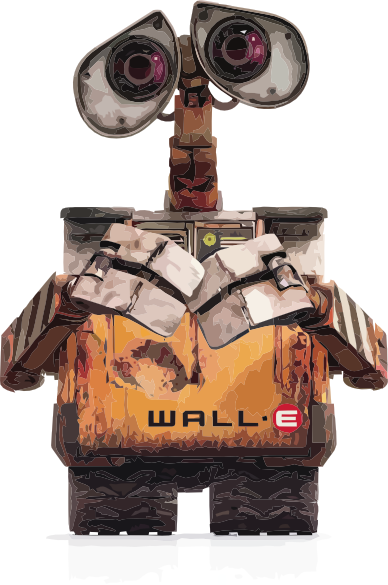
\includegraphics[width=\textwidth]{WallE}
%    \caption{Wall-E}
%    \label{fig:WallE}
%  \end{subfigure}             
%  \begin{subfigure}[b]{0.3\textwidth}
%    
\includegraphics[width=\textwidth]{minion}
%    \caption{Minions}
%    \label{fig:Minnion}
%  \end{subfigure}
%  \caption{Best Animations}
%  \label{fig:animations}
%\end{figure}


%\end{landscape}

%!TEX root = ../thesis.tex
%*******************************************************************************
%****************************** Third Chapter **********************************
%*******************************************************************************
\chapter{Reduced Order Modeling of Comb-Drive in Electrolytes}

% **************************** Define Graphics Path **************************
\ifpdf
    \graphicspath{{Chapter3/Figs/Raster/}{Chapter3/Figs/PDF/}{Chapter3/Figs/}}
\else
    \graphicspath{{Chapter3/Figs/Vector/}{Chapter3/Figs/}}
\fi

\section{Summary}
The focus of this chapter will be the development of reduced order models for the comb-drive actuator in electrolytes. We will first review the Poisson-Nernst-Planck equations for describing ionic liquids between parallel plates. This will be followed by a discussion of how these equations facilitate the conceptualization of the system as a circuit, and how this conceptualization was used to develop the classic model. In particular, the assumptions behind the classic model will be enumerated, as will it's shortcomings when fit to data. Finally, we will present our newly developed models, the assumptions behind this work, and opportunities for further work with regard to these models. 

\section{Poisson-Nernst-Planck (PNP) Equations}
We saw in Chapter 2 that modeling a comb-drive actuator in electrolytes reduces to modeling the overlapping regions of its fingers as parallel plates filled with a dilute ionic solution. This system is classically described by the Poisson-Nernst-Planck (PNP) equations. The one-dimensional PNP equations are

\begin{align}
    \frac{\partial c_\pm}{\partial t} = - D\frac{\partial}{\partial x}\bigg(-\frac{\partial c_\pm}{\partial x} \mp  \frac{ze}{k_B T}c_\pm \frac{\partial \phi}{\partial x}\bigg) \label{pnp_equations_1} \\
    -\epsilon \frac{\partial^2 \phi}{\partial x^2} = \rho_e = ze(c_+ - c_-) \label{pnp_equations_2} 
\end{align}
where $c_+$ and $c_-$ are the concentrations of the negative and positive ions respectively, $\phi$ is the electric potential, D is the diffusivity of the electrolyte, which is assumed to be constant throughout the domain, $z$ is the valence number of the electrolytes, $k_B$ is the Boltzmann constant, $T$ is the temperature of the domain, $\epsilon$ is the relative permittivity of the aqueous solution, $\rho_e$ is the electric charge density, and $e$ is the charge of an electron.

Before performing further analysis on the PNP equations, it is important that we do two things. First, we non-dimensionalize the PNP equations, and then we communicate the physical intuition of the resulting equations. We non-dimensionalize the PNP equations as was done by Druzgalski et al \cite{Druzgalski2013}. The potential, time, concentration, and spatial coordinates are non-dimensionalized as

\begin{equation}\label{nondim_quants}
    \phi^* = \frac{\phi}{V_T}, \quad t^* = \frac{Dt}{g^2}, \quad  c^*_0 = \frac{c}{c_0}, \quad  x^* = \frac{x}{g},
\end{equation}
where $V_T = \frac{k_B T}{e}$ is the thermal voltage, $g$ is the length of the gap between comb-drive fingers, $c_0$ is the bulk concentration of an ion, and the rest of the terms in the equation are defined after \ref{pnp_equations_1} and \ref{pnp_equations_2}. Using these terms, the non-dimensional form of the PNP equations is
\begin{align}
    \frac{\partial c_\pm^*}{\partial t^*} = - \frac{\partial}{\partial x^*}\bigg(-\frac{\partial c_\pm^*}{\partial x^*} \mp  c_\pm^* \frac{\partial \phi^*}{\partial x^*}\bigg) \label{pnp_equations_nondim_1} \\
    -2 \gamma^2 \frac{\partial^2 \phi^*}{\partial x^{*2}} = \rho_e^* = c_+^* - c_-^* \label{pnp_equations_nondim_2} 
\end{align}
where $\gamma = \frac{\lambda_d}{g}$. The summation in \ref{pnp_equations_nondim_1} is essentially the nondimensional current flux, $f_\pm^*$, of the positive and negative ions respectively.


\subsection{Circuit View of System using Linearized PNP Equations}
We have introduced and non-dimensionalized the PNP equations, as well as given physical intuition regarding its non-dimensional form. We will now use the non-dimensionalized PNP equations to explain the representation of electrolytes between parallel plates as a circuit. 

We first make the critical assumption that the voltage applied to the parallel plate is small. A small voltage is defined as a voltage that is at most the same order of magnitude as the thermal voltage, $V_T$, which is about 25 $\mV$. When the applied voltage is small, the region between the parallel plates is described as three distinct parts, figure \ref{conc_profile}. The center of the domain is called the bulk, and is characterized by an equal concentration of positive and negative ions, low concentration gradients, and a linear potential profile. The two regions located close to the parallel plates, however, are characterized by high concentration gradients, unequal amounts of positive and negative ions, and a nonlinear potential profile. The concentration of positive ions is much higher than the negative at the parallel plate with a lower potential, and vice versa at that with one that is higher. 

\begin{figure}[htpb]
    \begin{center}
    
\includegraphics[width=0.7\linewidth]{Chapter3/figure/conc_profile.png}
    \caption{Schematic of concentration profile of negative and positive ions of electrolyte between parallel plates.}\label{conc_profile}
    \end{center}
\end{figure}

We can apply the non-dimensional PNP equations to these three regions separately, and use the assumption of a small applied voltage, to develop a circuit model for the system. We start with the bulk region in which the concentration gradient is zero, $\frac{\partial c_\pm^*}{\partial x^*} = 0$, and the potential profile is linear, $\frac{\partial \phi^*}{\partial x^*}=a \implies \frac{\partial^2 \phi^*}{\partial x^{*2}}=0$, where $a$ is some constant. Using these assumptions, \ref{pnp_equations_nondim_1} and \ref{pnp_equations_nondim_2} reduce to

\begin{align}
    \frac{\partial c_\pm^*}{\partial t^*} = - \frac{\partial}{\partial x^*}\bigg( \mp  c_\pm^* \frac{\partial \phi^*}{\partial x^*}\bigg) = 0 \label{pnp_equations_simple_nondim_1} \\
    -\gamma^2 \frac{\partial^2 \phi^*}{\partial x^{*2}} = \rho_e^* = c_+^* - c_-^* = 0\label{pnp_equations_simple_nondim_2} 
\end{align}

So, in the bulk we can assume that the concentration of positive and negative ions are equal, and that the concentration does not change as a function of time. We can now write the net current flux in the system as
\begin{align}
    j = f_+^* - f_-^* & = (c_+^* + c_-^*)\frac{\partial \phi^*}{\partial x^*} \label{bulk_current_flux_1} \\ 
    & = 2c_0^*\frac{\partial \phi^*}{\partial x^*} \label{bulk_current_flux_2}  
\end{align}
where \ref{bulk_current_flux_2} is obtained by using the fact that $c_+^* = c_-^*=c_0^*=1$ in the bulk. Equation \ref{bulk_current_flux_2} has the form $I=\frac{V}{R}$. We can, therefore, view the non-dimensional resistance and voltage of the bulk region, respectively, as 

\begin{equation} \label{bulk_resist_volt}
    R_{Bulk}^* = \frac{1}{2c_0^*}, \quad V_{Bulk}^* = \int_{0}^{g} \frac{\partial \phi^*}{\partial x^*} dx^*.
\end{equation}

We can perform a similar analysis on the electric double layer regions between the parallel plates. In this region, the poisson equation is 
\begin{align}
    -\gamma^2 \frac{\partial^2 \phi^*}{\partial x^{*2}} & = c_+^* - c_-^* = \rho_e^* \label{poisson_nondim_cap_1} \\
    &  = \text{sinh}(\frac{\phi^*}{2}) = \frac{dq^*}{dx^*}\nonumber
\end{align}
where \ref{poisson_nondim_cap_1} is obtained by assuming a boltzmann distribution.
\begin{equation} \label{boltzmann_distrib}
    c_+^* = c_0^* e^{-\frac{\phi z e}{k_B T}}, \quad c_-^* = c_0^* e^{\frac{\phi z e}{k_B T}}
\end{equation}
 Under the assumption of linearity, we rewrite \ref{poisson_nondim_cap_1} as  
\begin{equation}\label{poisson_nondim_ode}
\gamma^2 \frac{d^2\phi^*}{dx^{*2}} - \phi^* =0.
\end{equation}.
Solving this ODE, and taking a first order derivative of it's solution, yields
\begin{equation} \label{poisson_nondim_odesol}
\frac{d\phi^*}{dx^*} = -\gamma^{-1} \phi^*,
\end{equation}
We now rewrite \ref{poisson_nondim_cap_1}, using the solution of \ref{poisson_nondim_ode}, as
\begin{equation} \label{poisson_nondim_odesol_charge}
-2 \bigg(\frac{\lambda_d}{g}\bigg)^2 \frac{d^2\phi^*}{dx^{*2}} = -2 \phi^* = \frac{dq^*}{dx^*}
\end{equation}
Equations \ref{poisson_nondim_odesol} and \ref{poisson_nondim_odesol_charge} indicate that the boundary regions between the electrolytes can be represented as a capacitor. We obtain the dimensionless linear differential capacitance of this region by taking the quotient of \ref{poisson_nondim_odesol} and \ref{poisson_nondim_odesol_charge}, yielding
\begin{equation} \label{lin_diff_cap}
\frac{dq^*}{dx^*}\frac{dx^*}{d\phi^*} = \frac{dq^*}{d\phi^*} = 2\frac{\lambda_d}{g} = 2\gamma = C_0 
\end{equation}

Based on this analysis, it is clear that we can view electrolytes between parallel plates as a circuit composed of boundary oxide capacitors, and a bulk resistor, figure \ref{classic_circuit}.

\section{Classic Circuit Model of Comb-Drive Actuator in Electrolyte}
In this section, we will discuss the classic model of the comb-drive in electrolytes, which is based on the circuit model derived in the previous section, figure \ref{classic_circuit}.

\begin{figure}[htpb]
    \centering
    \begin{minipage}{\textwidth}
        \centering
        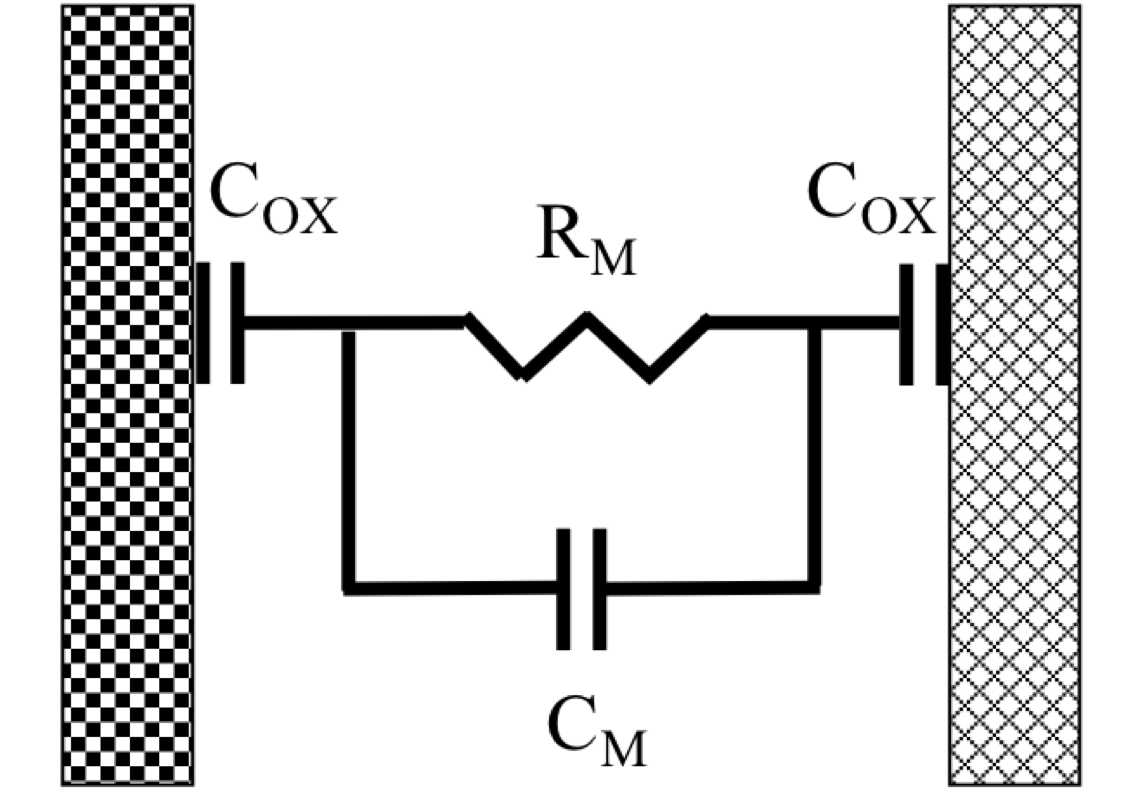
\includegraphics[width=0.6\textwidth]{Chapter3/figure/classic_circuit.png} % first figure itself
        \caption{Circuit schematic of the classic circuit model for describing a comb-drive actuator in electrolytes. It is composed of an oxide capacitor at the boundary, and a parallel resistor/capacitor in the bulk.}\label{classic_circuit}
    \end{minipage}\vfill
    \begin{minipage}{\textwidth}
        \centering
        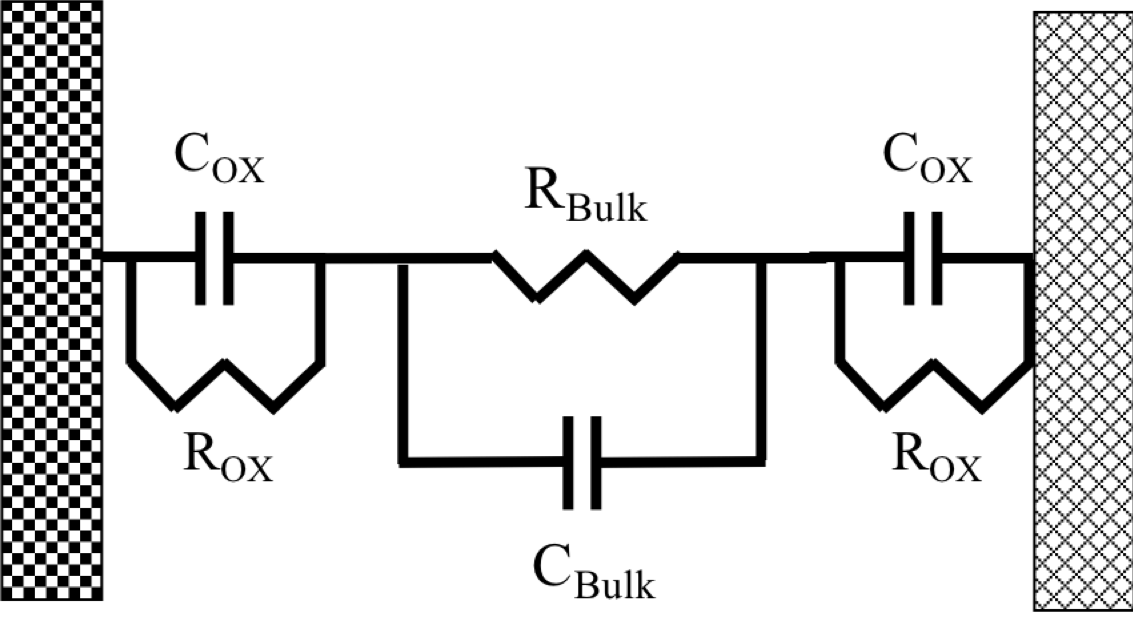
\includegraphics[width=0.8\textwidth]{Chapter3/figure/leaky_ox_circuit.png} % second figure itself
        \caption{Circuit schematic of the leaky circuit model for describing a comb-drive actuator in electrolytes. In this case the boundary is composed of a parallel resistor and capacitor to represent the oxide.}\label{leaky_ox_circuit}
    \end{minipage} \vfill
    \begin{minipage}{\textwidth}
        \centering
        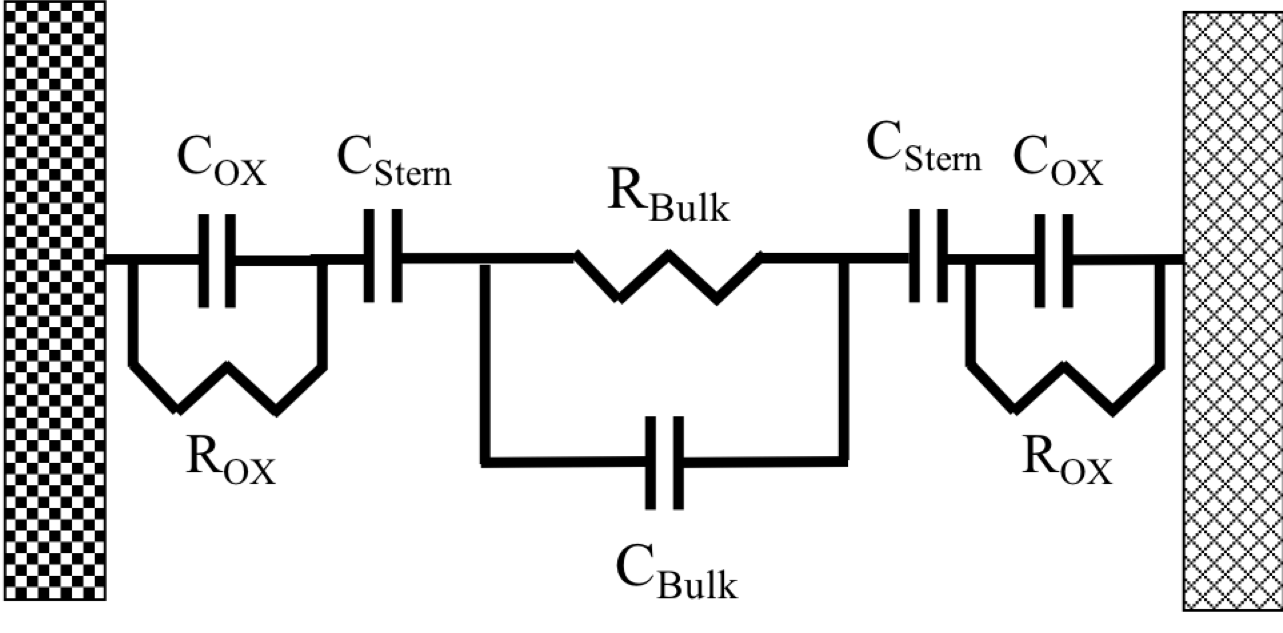
\includegraphics[width=0.8\textwidth]{Chapter3/figure/leaky_ox_stern_circuit.png} % second figure itself
        \caption{Circuit schematic of the leaky circuit model for describing a comb-drive actuator in electrolytes. It is similar to the leaky oxide schematic, except a stern layer is placed in series with the oxide resistor/capacitor.}\label{leaky_ox_stern_circuit}
    \end{minipage} \vfill
\end{figure}

\begin{comment}
\begin{figure}[htpb]
    \begin{center}
    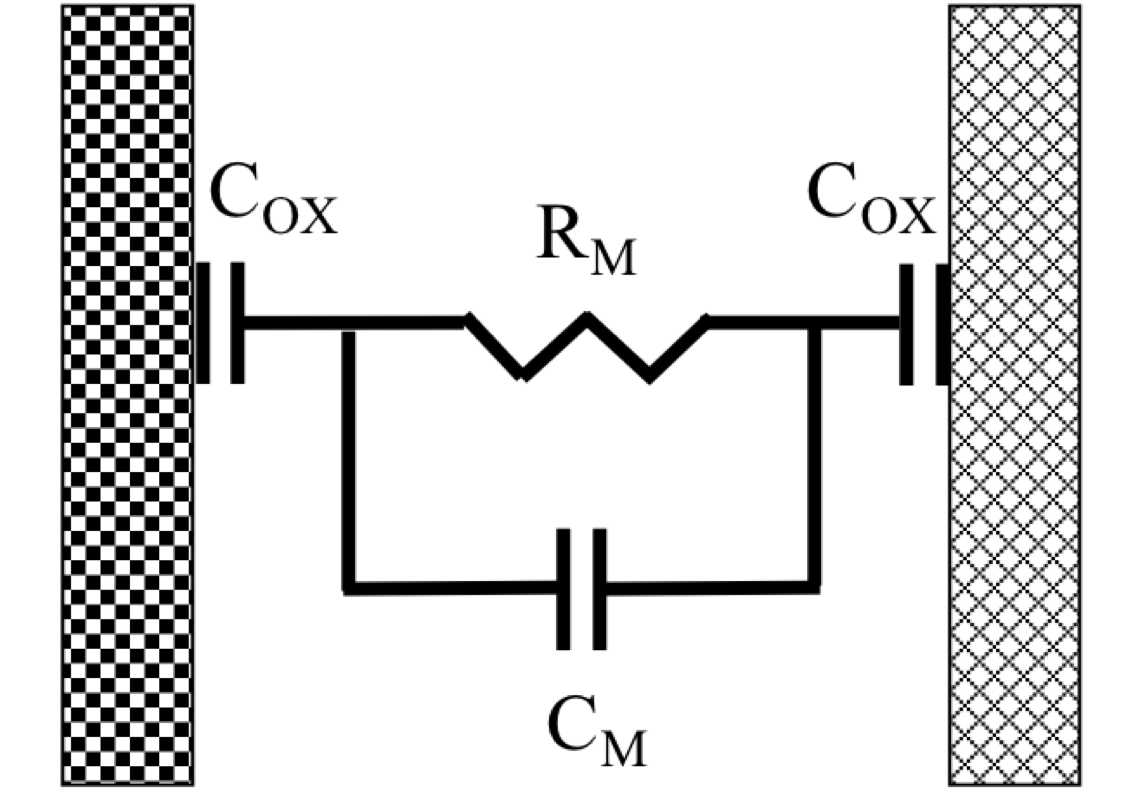
\includegraphics[width=0.7\linewidth]{Chapter3/figure/classic_circuit.png}
    \caption{Circuit schematic of the classic circuit model for describing a comb-drive actuator in electrolytes. It is composed of an oxide capacitor at the boundary, and a parallel resistor/capacitor in the bulk.}\label{classic_circuit}
    \end{center}
\end{figure}
\end{comment}

The force, $F$, experienced by a comb-drive actuator in air can be calculated as
\begin{equation}\label{air_force_comb} 
F = kx = \dfrac{Nb\epsilon_0}{g}V_{App}^2,
\end{equation}
where \textit{k}, the stiffness of the comb-drive, \textit{x}, its displacement, \textit{N}, the total number of comb-pair fingers, \textit{b}, the comb finger thickness (into the page), and \textit{g}, the distance between overlapping fingers, are properties of the comb-drive.  $\epsilon_0$ is the permittivity of free space, and $V_{App}$ is the voltage applied to an overlapping pair of fingers. In this scenario, fringe effects of the comb-drive tip can be ignored. This simplified model is most accurate with sufficient overlap between fingers\cite{Ye1998}. The classic model constructed by Mukundan et al. and Panchawagh et al. can be expressed by modifying \ref{air_force_comb} \cite{MukundanandPonce2009,Panchawagh2009},
\begin{equation}\label{classic_force_comb}  
F = \dfrac{Nb\epsilon_0\epsilon_W}{g}f(\omega)V_{AppRMS}^2 = \dfrac{Nb\epsilon_0\epsilon_W}{g}f(\omega)\bigg(\dfrac{V_{App}}{\sqrt[]{2}}\bigg)^2,
\end{equation}
where $V_{AppRMS}$ is the root-mean-square of the applied voltage, $\epsilon_W$ is the relative permittivity of water, and $f(\omega)$ is a function of the applied frequency that is equal to \cite{MukundanandPonce2009,Panchawagh2009}
\begin{equation} \label{classic_frequency_eqn}
f(\omega) = \bigg|\dfrac{Z_{Bulk}}{Z_{Bulk}+2*Z_{Interface}(\omega)}\bigg| ^2, \quad Z_{Interface}=Z_{Ox}.
\end{equation}
Here $Z_{Bulk}$ is the impedance of the bulk resistor, and $Z_{Interface}$ the impedance of the interface between the bulk electrolyte and the electrode. In this case, $Z_{Interface}$ is equivalent to $Z_{Ox}$, the impedance of the native oxide capacitor. These impedances are expressed as 
\begin{equation} \label{bulk_oxide_impedances}
Z_{Bulk} = R_{Bulk}, \quad Z_{Ox} = \dfrac{1}{j\omega C_{Ox}}.
\end{equation}
We note that $C_{Bulk}$ is ignored, because $C_{Ox}$ dominates the capacitive behavior in the range of frequency we consider. From equations \ref{classic_force_comb}-\ref{classic_frequency_eqn}, the time-constant that governs the frequency required to overcome ionic shielding, and facilitate actuation, is \cite{MukundanandPonce2009,Panchawagh2009}
\begin{equation} \label{classic_timeconst}
\tau = R_{Bulk}C_{Ox}.
\end{equation}
At higher concentrations the bulk resistance, $R_{Bulk}$, decreases so higher frequencies of applied voltages are required to overcome shielding, and facilitate actuation. 

\subsection{Assumptions and Validity of Classic Circuit Model}
The classic model, while a major breakthrough in modeling electrostatic comb-drive actuators in electrolytes, makes three major assumptions: i) that the native oxide is a pure dielectric, ii) that the ion concentration of the bulk electrolyte is constant, and iii) that the Stern layer can be neglected compared to the oxide layer. Figure \ref{classic_circuit_fit} shows the displacement of a comb-drive actuator in KCl at concentrations of 0.1 mM, 0.5 mM, and 1 mM respectively. We see that, while the Classic model accurately captures the trend of displacement, it tends to significantly underestimate the displacement in the low frequency region, and overestimate it in the intermediate frequency regions. 

In order to overcome these shortcomings, we develop a hierarchy of novel models that addresses assumptions i)-iii) both individually and in concert. Subsequently, we select the simplest model that explains the comb-drive displacement in electrolytes. The developed models are 1) Leaky Oxide, 2) Leaky Oxide + Stern, 3) Variable Resistor, and 4) Leaky Oxide + Stern + Variable Resistor models. These models, as well as the assumptions of the Classic Circuit model that they address, are listed in Table \ref{hiearchy_table}. We find that the model which removes assumptions i) and ii) is sufficient to accurately predict the displacement of a comb-drive actuator in electrolytes.


\begin{figure}[htpb]
    \begin{center}
    \includegraphics[width=0.7\linewidth]{Chapter3/figure/placeholder.png}
    \caption{Placeholder for classic model fit to comb-drive actuator displacement data at 0.1 mM, 0.5 mM, and 1 mM $KCl$ respectively}\label{classic_circuit_fit}
    \end{center}
\end{figure}

\begin{table}[!htb]
\begin{center}
{\begin{tabular}{|c|c|}
	\hline
	\textbf{Model (i)} & \textbf{Classic Model} \\
     &  \textbf{Assumptions Removed} \\
    \hline
    Leaky Oxide (1) & i) Pure Dielectric Oxide\\
    \hline
    Leaky Oxide  & i) Pure Dielectric Oxide \\
    + Stern (2)    & ii)  No Stern layer \\
    \hline
    Variable Resistor (3) & iii) Constant Bulk Resistor \\
    \hline
    Leaky Oxide+ & i) Pure Dielectric Oxide\\
    Stern+   & ii)  No Stern layer \\
     Variable Resistor (4) & iii) Constant Bulk Resistor  \\
    \hline  
\end{tabular}}
\caption{Hierarchy of models developed in this paper, and the classic circuit model assumptions they address}\label{hiearchy_table}
\end{center}
\end{table}


\section{Novel Circuit Models of Comb-drive Actuator in Electrolytes}
In this section, we outline the development of the set of models summarized in table \ref{hiearchy_table}. In order to represent these models, we re-express the frequency dependence of the force on the comb-drive actuator, \ref{classic_force_comb}, as
\begin{equation}\label{general_red_force_comb}
F = \dfrac{Nb\epsilon_0\epsilon_W}{g}h_i(\omega)V_{AppRMS}^2
\end{equation}
where $h_i$ is the function of frequency that corresponds to the Leaky Oxide, Leaky Oxide + Stern, Variable Resistor, and Leaky Oxide + Stern + Variable Resistor models (i=1,2,3,4). Explicitly, 

\begin{align}\label{gen_freq_eqn}
h_i(\omega) = \bigg|\dfrac{Z_{Bulk}}{Z_{Bulk}+2*Z_i(\omega)}\bigg|^2,  i=1,2,3,4,5
\end{align}

The Leaky Oxide and Leaky Oxide + Stern models yield analytical expressions for $h_i$, while the frequency dependence of the Variable Resistor and Leaky Oxide + Stern + Variable Resistor models are evaluated numerically, after solving systems of ordinary differential equations (ODEs). 
 
The Leaky Oxide and Leaky Oxide + Stern models are created by modifying the interface impedance, $Z_i, i=2,3$. Figures \ref{classic_circuit}, \ref{leaky_ox_circuit}, and \ref{leaky_ox_stern_circuit} shows the circuit model for the Classic, Leaky Oxide, and Leaky Oxide + Stern models. For both the Leaky Oxide, and Leaky Oxide + Stern models, the bulk impedance is a constant value resistor, $Z_{Bulk}=R_{Bulk}$. However, their interface impedances vary. Noting that the leaky oxide and stern layer impedances are 

\begin{equation} \label{oxide_stern_impedances}
Z_{Ox} = \frac{R_{Ox}}{1+j\omega R_{Ox}C_{Ox}}, \quad Z_{Stern} = \frac{1}{j\omega C_{Stern}},
\end{equation}

we can right the interface impedance of the Leaky Oxide + Stern model, and the Leaky Oxide models as 

\begin{align}
Z_{LeakyOx}(\omega) = Z_{Ox}, \label{leaky_ox_imped} \\ 
Z_{LeakyOx+Stern}(\omega) = Z_{Ox}+ Z_{Stern}  \label{leaky_ox_stern_imped}. 
\end{align}

The Variable Resistor and Leaky Oxide + Stern + Variable resistor models are modifications of the Classic and Leaky Oxide + Stern models respectively. Specifically, both of these models remove the assumption that the bulk resistance is constant, and instead model it as a function of bulk concentration. In addition, these models account add the stern layer, and the nonlinear electric double layer to the interface. We note that it is assumed that the concentration in the bulk changes in a manner that is spatially homogeneous. This yields a system of ODEs of the form,

\begin{align} \label{ode_states}
\dot{\mathbf{y}} = f(\mathbf{y},t,\omega), \nonumber\\ \mathbf{y} =[q^*,V_{Ox}^*,V_{St}^*,V_{EDL}^*,V_{Bulk}^*,i^*,c_0^*,R_{Bulk}^*]^T
\end{align}

where  $q$ is the surface charge on the Electric Double Layer (EDL) capacitor, $V_{Ox}^*$  is the voltage drop across the native oxide, $V_{Stern}^*$ is the voltage drop across the stern layer, $V_{EDL}^*$ is the voltage drop across the EDL, $V_{Bulk}^*$ is the voltage drop across the bulk, $i^*$ is the current, $c_0^*$ is the concentration of the bulk electrolyte, and $R_{Bulk}^*$ is the resistance of the bulk. All of these quantities are dimensionless,  and $V_{Bulk}^*$ is re-dimensionalized to $V_{Bulk}$ when evaluating displacement. The ODEs for the Leaky Oxide + Stern + Variable Resistor model are of the same form as equation (7).

The main difference between these models is in the modification of $V_{Ox}^*$ to account for the parallel addition of $R_{Ox}$ to $C_{Ox}$, figures \ref{leaky_ox_circuit}. Unlike for the case of the Leaky Oxide and Leaky Oxide + Stern models, evaluating the functional dependence on force, $h_i(\omega)$, requires numerical integration. Specifically, we use the RMS integral of $V_{Bulk}$ to obtain

\begin{align} \label{numeric_vrms}
V_{RMS}(\omega) = \sqrt[]{\frac{1}{T} \int_{0}^{T}V_{Bulk}(\omega,t)^2dt} = h_i(\omega)V_{AppRMS},\nonumber\\ i = 3,4
\end{align}

\subsection{ODEs for Numeric Circuit Models}
We have introduced abstractly the Variable Resistor, and the Leaky Oxide + Stern + Variable Resistor models. In this section, we enumerate the non-dimensional ODEs that must be solved in order to evaluate these models. For the variable resistor model, the system of ODEs is

\begin{align}
\frac{dq^*}{dt^*} = i^* \label{charge_state} \\
\frac{dV^*_{EDL}}{dt^*} = \frac{i^*}{C_{EDL}^*} \label{vedl_state} \\%\frac{i}{dq/dV_{EDL}} \\
\frac{dV^*_{Stern}}{dt^*} = \frac{i^*}{C_{Stern}^*} \label{vstern_state} \\%\frac{i}{ \frac{C_{Stern} \lambda_{D}}{C_{Water} \lambda_{Stern}}dq/dV_{0}} \\
\frac{dV^*_{Ox}}{dt^*} = \frac{i^*}{C_{Ox}^*} \label{vox_state} \\
\frac{dc^*_0}{dt^*} = -2i^*sign(q^*) \label{concentration_state}\\
\frac{dR^*_{Bulk}}{dt^*} = \frac{-1}{2c_{0}^{*2}}\frac{dc^*_0}{dt^*} \label{resistor_state}\\
\frac{dV^*_{Bulk}}{dt^*} = \frac{di^*}{dt^*}R^*_{Bulk} + i^*\frac{dR^*_{Bulk}}{dt^*}\label{vbulk_state}  \\ 
\frac{di^*}{dt^*} = \frac{\bigg(\frac{dV^*_{Bulk}}{dt^*}-2\frac{d}{dt^*}V^*_{INT}-i^*\frac{dR^*_{Bulk}}{dt^*}\bigg)}{R^*_{Bulk}} \label{current_state} 
\end{align}
where 
\begin{equation}
    V^*_{INT}  = V^*_{EDL}+V^*_{Stern}+V^*_{Ox}   
\end{equation}
 and each state has been defined in the paragraph following \ref{ode_states}. $C_0$ is the dimensionless linear differential capacitance of the electric double layer, \ref{lin_diff_cap}, and $C_{EDL}$ is the dimensionless nonlinear differential capacitance of the electric double layer which is expressed as
\begin{equation} \label{edl_nonlinear}
C_{EDL} = C_{0} cosh\bigg(\frac{V^*_{EDL}}{2}\bigg).
\end{equation}

We note four things. First, the differential equation for the bulk resistor, $R_{Bulk}^*$ is obtained by taking a time derivative of the bulk resistance expressed in \ref{bulk_resist_volt}. Second, with the exception of the $C_{EDL}^*$, the non-dimensional capacitance of circuit element $l$, $C_l^*$, is 

\begin{equation}
    C_l^* = \bigg(\frac{C_{l} \lambda_{D}}{C_{Bulk} \lambda_{l}}C_0\bigg)
\end{equation}
where $C_{l}$ is the dimensional capacitance of the circuit element, $C_{Bulk}=\frac{\epsilon_W}{g}$ is the capacitance of the bulk which is assumed to be calculated based on the relative permitivitty of water, $\lambda_{l}$ is the thickness of the physical layer represented by circuit element $l$, and $\lambda_{D}$ is the debye lenght. Third, the voltages in this system are where non-dimensionalized using the thermal voltage, $V_T$. Finally, the voltage, $V_{l}$, bulk resistor, $R_{Bulk}^*$, capacitances, $C_l^*$, and time $t^*$ are the only parts of the ODE that are explicitly non-dimensionalized. The non-dimensional charge and current fall out of solving the ODEs with these quantities.

The system of ODEs for the Leaky Oxide + Stern + Variable Resistor model is identical to that of the Variable Resistor model, with the exception of a modification to \ref{vox_state} which is rewritten as
\begin{align} \label{vox_state_leakoxstern}
\frac{dV^*_{Ox}}{dt^*} = \frac{i^* - V^*_{Ox}/R^*_{Ox}}{C^*_{Ox}};
\end{align}

\section{Neglected Effects of Novel Models}
Up until this point, we have neglected two key effects in the development of our models. The first is the depletion layer that can develop in doped silicon, and the second is the formation of concentration gradients in the bulk electrolyte. We describe both of these effects in this section, and justify their explicit absence from our models. 

\subsection{Depletion Layer Formation}
The silicon wafers used to fabricate the comb-drive actuators are p-type boron-doped to 0.008-0.01 \textOmega $\textrm{ }cm$. When a voltage is applied to the comb-drive, the resulting external electric field causes charge carriers to collect at the interface of the silicon and native oxide. This region is called the depletion layer, and can also be approximated as a capacitor. The relative importance of this capacitance, compared to other circuit elements in our models, is determined by the width of the depletion layer. We perform a scaling analysis in order to determine the importance of this depletion layer.

Figure \ref{depletion_layer} depicts the depletion layer in series with the native oxide and Stern layers, as well as the bulk electrolyte, for a single comb-drive finger. The analysis detailed in this section assumes that the native oxide is a pure dielectric, and makes use of dimensional quantities. We write Poisson's equation for the depletion layer as
\begin{equation}
\frac{d^2\phi}{dx^2} = -\frac{dE}{dx} = -\frac{e}{\varepsilon_{Si}}(n_+ - n_- + N_d), \quad -x_d \leq x \leq 0
\end{equation}
where $n_+$ and $n_-$ are positive and negative free charge carrier concentrations respectively, and $N_d$ is the concentration of the positive dopant. We solve for the electric field, assuming that there are no free charge carriers in the depletion layer.
\begin{equation} 
E(x) = \frac{eN_d(x+x_d)}{\varepsilon_{Si}}.
\end{equation}
We next require that the electric field be continuous at the interface of the native oxide and the depletion layer, $x=0$. and solve for the depletion layer width, $x_d$.

\begin{figure}[htpb]
    \begin{center}
    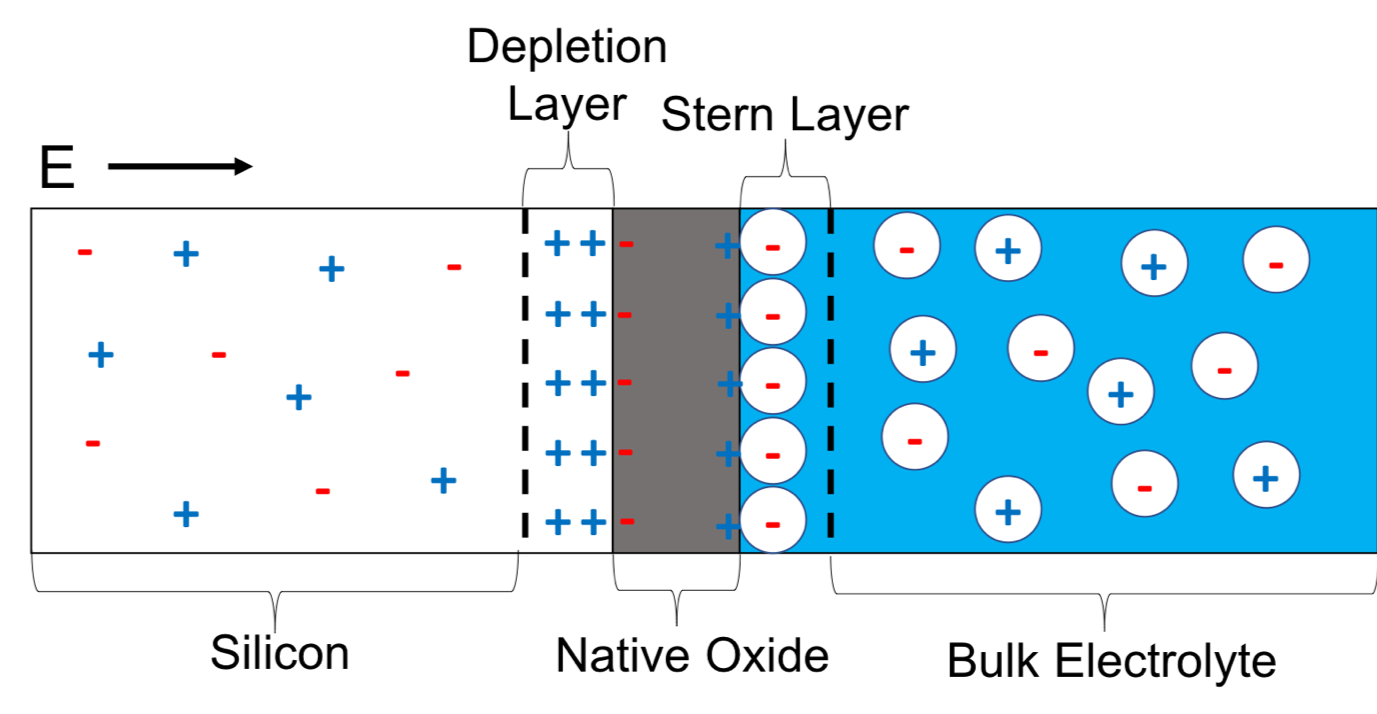
\includegraphics[width=0.7\linewidth]{Chapter3/figure/depletion_layer.png}
    \caption{Illustration of one finger in a pair of comb-drive fingers. It depicts the Silicon substrate, the depletion layer, the native oxide, the Stern Layer, and the bulk electrolyte.}\label{depletion_layer}
    \end{center}
\end{figure}
% \begin{equation}
% E(x=0) = \frac{eN_dx_d}{\varepsilon_{Si}} = \frac{V_{Ox}}{t_{Ox}}.
% \end{equation}
% Re-writing equation (52) allows us to write the depletion layer width as
\begin{equation}
x_d = \frac{\varepsilon_{Si}}{t_{Ox}}\frac{V_{Ox}}{eN_{d}}.
\end{equation}
If we use the nominal values of the physical parameters in equation (51), shown in \ref{table_phys_param_nomvals}, then the depletion layer width is 
\begin{equation}
x_d = 3 \times 10^{-8} V_{Ox}.
\end{equation}
We know that $V_{Ox}$ is at most O(1), so we can approximate the minimum capacitance of the depletion layer as
\begin{equation}
C_{D} \approx \frac{\varepsilon_0 \varepsilon_{Si}}{x_d} = 0.0034 
\end{equation}

\begin{table}[!htb]
\begin{center}
{\begin{tabular}{|c|c|}
	\hline
	\textbf{Physical Parameters} & \textbf{Nominal Values} \\
    \hline
    $\varepsilon_{Si}$ & 11.68 \\
    \hline 
    $t_{Ox}$ & 2 $nm$ \\
    \hline
    $N_d$  & $10^{25} m^{-3}$  \\
    \hline
\end{tabular}}
\caption{Nominal values of physical parameters used for approximated the width of the depletion layer.}\label{table_phys_param_nomvals}
%\begin{flushleft} 
%Table III: 
%\end{flushleft} 
\end{center}
\end{table} 

Since the nominal capacitance of the Stern and native oxide layers are O(0.1) and O(0.01) respectively, it is clear that the effects of the depletion layer capacitance is significant. While this is relevant for conceptualizing the physical system, explicitly modeling the depletion layer does not impact the ability of our reduced models to fit the data. The models presented in this chapter are lumped circuit models, rather than spatial models. As a result, the depletion layer capacitance, which is in series with the Stern or oxide layer capacitance depending on the model, can be lumped in with the capacitance of these layers. When these models are fit, the resulting value of the Stern and oxide capacitance  should be viewed as compensating for both these respective layers and the Depletion layer.

\subsection{Concentration Gradients}
The variable resistor models described in the previous section assumes that the concentration of the electrolytes changes uniformly across the bulk electrolyte, i.e. that the concentration has no gradients. While this is not generally true, the impact of concentration gradients is only relevant when large low-frequency voltages are applied to the bulk. In the case of the comb-drives fabricated for this paper, we postulated that the impedance of the native oxide at low frequencies was sufficiently high enough to prevent this. We confirm in the next chapter that, in the context of our current devices, the variable resistor models that account for concentration gradients fit the data identically to our models that assume uniform concentration. For the sake of completeness, we illustrate here how we account for concentration gradients in our variable resistor model. This derivation is derived based on the work of Bazant et al \cite{Bazant2004}.

Bazant et al. used matched asymptotics to derive expressions for the change in the concentration of a \textit{z:z} electrolyte. They first expressed the dimensionless concentration in the bulk as
\begin{equation} \label{concentration_asympt}
c^* = c_+^* + c_-^* = 2c_0^* + \gamma c_1^*
\end{equation}
where $c_1^*$ accounts for the variation in the bulk concentration, and $\gamma$ is as defined in \ref{lin_diff_cap}. The time derivative of the the bulk concentration is then
\begin{equation} \label{dcdt_asympt}
\frac{dc^*}{dt^*} = \gamma \frac{dc_1^*}{dt^*} = \gamma \frac{d^2c_1^*}{dx^{*2}},
\end{equation}
with the boundary condition
\begin{equation} \label{dcdt_asympt_bc}
\frac{dc_1^*}{dx^*}(x=0,t) = -2 sinh\bigg(\frac{V_{EDL}^*}{2}\bigg) \frac{dV_{EDL}^*}{dt^*}.
\end{equation}
In order to account for the concentration gradient, we replace \ref{concentration_state} with \ref{dcdt_asympt} and \ref{dcdt_asympt_bc}. We finally replace $R_{Bulk}^*$ and $\frac{dR_{Bulk}^*}{dt^*}$ with
\begin{equation}
R_{Bulk}^* = \frac{1}{c^*},
\end{equation}

and 

\begin{equation}
\frac{dR_{Bulk}^*}{dt^*} = \int_{0}^{g^*} \frac{-1}{c^{*2}}\frac{dc^*}{dt^*}dx^*.
\end{equation}
respectively.

\section{Chapter Review and Further Work}
In this chapter, we justified the use of a circuit model to describe the behavior of electrolytes between parallel plates using the PNP equations, detailed the classic circuit model that falls out of this circuit model, as well as the assumptions behind this model, and presented a hierarchy of models that addressed the assumptions of the classic circuit model. Moreover, we noted important effects neglected by our reduced models, and stated that, as will be shown in chapter 4, that these had no impact on describing the comb-drive actuators in electrolytes that were fabricated for this dissertation.

In the future, it would be useful to numerically, and experimentally, explore how changes in the parallel plate system, especially the thickness of the native oxide, would impact the importance of effects neglected by our model.
%!TEX root = ../thesis.tex
%*******************************************************************************
%****************************** Third Chapter **********************************
%*******************************************************************************
\chapter{Validating Reduced Order Models}

\ifpdf
    \graphicspath{{Chapter4/Figs/Raster/}{Chapter4/Figs/PDF/}{Chapter4/Figs/}}
\else
    \graphicspath{{Chapter4/Figs/Vector/}{Chapter4/Figs/}}
\fi

\section{Summary}
This chapter focuses on validating the hierarchy of models developed in Chapter 3. In the context of this work, model validation is the process of both estimating the parameters of models in such a way that they simultaneously minimize the difference between these models and experimental data, and give reasonable uncertainty in the model output and estimated parameters.

The chapter begins with a formulation of parameter estimation as a nonlinear optimization problem, followed by a discussion of different methods of optimization, with an emphasis on Particle Swarm Optimization (PSO), a review of challenges in optimization, and a discussion about how uncertainty of parameters can be quantified through confidence regions. We wrap up the algorithmic component of our discussion by presenting a novel optimization framework that is used to simultaneously validate models, establish confidence in our results, and determine the number of experiments needed to yield a user-defined balance of fitting models with a high degree of accuracy, and giving a meaningful distribution of estimated parameters and model outputs. Subsequently, we present a two part discussion on the results of our novel algorithm when applied to our reduced comb-drive actuator in electrolyte models, and the accompanying experiments. The first part of the discussion, focuses on observing the results of our algorithm in the scenario where we are concerned only with determining which of the reduced models fit the data with the greatest degree of fidelity. In this part of the discussion, we make use of all our experiments, and comment on the simplest model that best fits the data. The second part of our discussion examines the results of our algorithm more holistically. Here, we observe the confidence regions found by our algorithms when applied to different reduced order models, at different numbers of experiments and measurements. We then comment on how the confidence regions, as well as the distribution of model outputs, change for each model as a function of the amount of data used in the fit, and at a particular confidence, $1-\alpha$. Finally, we discuss how we can use the in-depth results of our algorithm to select the correct combination of reduced order models, and amount of data that allows us to explain the behavior of the comb-drive actuator with some balance of fit to data, and an appropriate distributions of model outputs and estimated parameters. 

\section{Parameter Estimation as an Optimization Problem}
The problem of estimating the parameters of a model that best fits the data can be represented as the following nonlinear optimization problem

\begin{equation} \label{orig_optim_problm}
\begin{aligned}
& \underset{x}{\text{minimize}}
& & y(\mathbf{x},\mathbf{z}) = y(\mathbf{x}) = ||\mathbf{f}(\mathbf{x},\mathbf{z}) - \mathbf{g}(\mathbf{z})||_p \\
& \text{subject to}
& & x_{i,min} \leq x_i \leq x_{i,max} , \; i = 1, \ldots, m.
\end{aligned}
\end{equation}

where $\mathbf{x}$ is the vector of tune-able parameters that the model takes as in input, $\mathbf{z}$ is the vector of inputs to the model that are not tune-able, $\mathbf{f}$ is the vector of values that are output by the model given a particular set of $\mathbf{x}$ and $\mathbf{z}$, $\mathbf{g}$ is the vector of values that are output given $\mathbf{z}$, $p$ is an integer that indicates the type of norm we are taking (eg. $p=1 \implies \textrm{ L1 norm}$), $x_i$ is the $i_{th}$ component of the vector $\mathbf{x}$, and $m$ is the number of components in that vector. This is a standard bounded nonlinear optimization problem. In our case, we bound the parameters of the model, $\mathbf{x}$, so that our optimization framework only selects physically realizable values, and we select $p=2$ so that the above objective function becomes L2 (least-squares).

\section{Optimization Techniques}
This section focuses on reviewing different optimization techniques. We discuss gradient methods, with a focus on the trust region reflective algorithm, and stochastic methods, with a focus on particle swarm optimisation. 

\subsection{Gradient Methods}

Gradient methods for optimization are among the most popular in literature. These methods use the gradients, or approximate gradients, of functions with respect to their tuneable inputs in order to find the value of these inputs that minimize or maximize said function. The most common gradient optimization method is gradient descent, which has gained particular favor in the machine learning community \textbf{CITE NG}. Given the optimization problem, \ref{orig_optim_problm}, and neglecting the constraints, gradient descent involves making an initial guess at the solution, $\mathbf{x}^{0}$, and iterating on that guess using,

\begin{equation} \label{grad_descent}
    \mathbf{x}^{n+1} = \mathbf{x}^{n} - \alpha g, \quad g = \nabla_\mathbf{x} y(\mathbf{x}^{n},\mathbf{z})
\end{equation}
where $\alpha$ is the learning rate, $x^{n}$ is the guess of the solution at the $nth$ iteration of gradient descent, $x^{n+1}$ is the guess at the $(n+1)th$ iteration based on the gradient of the objective function, and $\nabla_\mathbf{x} y(\mathbf{x}^{n},\mathbf{z})$ is the numeric or analytic gradient of $y$ with respect $\mathbf{x}$, evaluated at $\mathbf{x}^{n}$. While gradient descent is a powerful optimization method, it can be very expensive, especially when optimizing a nonlinear function. In particular, while the gradient moves in the direction of greatest change in the function, it does so at an arbitrary distance, making it more prone to "overreacting" to local curvature in a nonlinear function \textbf{illustration of this}.

In order to address this issue, a class of gradient based methods, termed Trust Region, methods were developed. These optimization methods in particular involve first determining the maximum magnitude, $\delta$, of change that can be imposed on the current guess of the solution. The size of $\delta$ is determined primarily by the extent to which the objective function being minimized reduces in the region around the current guess of a solution. There are a variety of algorithms for implementing this class of algorithms, the details of which are illustrated by Yuan et al., \textbf{CITE TRUST REGION}. To end our discussion on gradient methods, we will outline the general trust region problem.

The first step of the Trust-Region algorithm is making a local quadratic approximation of the objective function.

\begin{equation} \label{quad_approx}
    \tilde{y}(\mathbf{x}+\delta,\mathbf{z}) = y(\mathbf{x},\mathbf{z}) + g^T \delta + \delta^T B \delta 
\end{equation}
where g is as defined in \ref{grad_descent}, $\delta$ is some perturbation to $\mathbf{x}$, and $B$ is an approximation of the hessian of the objective function.\textbf{CITE TRUST REGION} If Like gradient descent, the Trust Region Algorithm is iterative. It selects a vector step by which to change $\mathbf{x}^n$ by using \ref{quad_approx} to solve the following constrained optimization problem,

\begin{equation} \label{trust_region_optim_problm}
\begin{aligned}
& \underset{\delta}{\text{minimize}}
& & y_n(\mathbf{x}^n,\mathbf{z}) + g_n^T \delta + \delta^T B_n \delta\\
& \text{such that}
& & ||\delta||_2 \leq \Delta_n.
\end{aligned}
\end{equation}

where $g_n$ is the gradient of the objective function evaluated at $\mathbf{x}^n$, $B_n$ is the approximation of the Hessian at the $\mathbf{x}^n$, and $\Delta_n$ is the trust region at iteration $n$. The size of $\Delta_n$ is determined by the extent to which the objective function, $y$, can be minimized within this region. If on the previous iteration, $n-1$, the objective function is sufficiently reduced, then the trust region generally expands. If not, it reduces. Since we simply use a Python implementation of the Trust Region Algorithm, we do not go into specifics. Details on a variety of Trust Region Algorithms can be found in Yuan et al, \textbf{CITE TRUST REGION}.  

\subsection{Stochastic Optimization Methods: Particle Swarm Optimization (PSO)}
Gradient based methods have two main limitations. The first is that they require the calculation of gradients, which can be expensive, and the second is that they are prone to local minima when given poor initial conditions. Stochastic optimization methods attempts to address both of these issues. Rather than taking gradients, stochastic optimization methods randomly search the solution space in order to minimize an objective function. Some of these algorithms have heuristically been shown to be more efficient at finding the global minimum of an objective function, \textbf{CITE PSO Thesis}. The stochastic optimization method of interest to us is Particle Swarm Optimization (PSO). In this section we will review PSO, and its key variants.  

The basic version of PSO was developed by Kennedy et al. \textbf{Cite Basic PSO Paper}. In this version of PSO, the user initializes a "swarm" of $m$ guesses at an optimal solution, $(\mathbf{x}_1,...,\mathbf{x}_m)$, and evaluates the function at each of these guesses. The guess that results in the most optimal function, $\mathbf{x}_{Best}$, is stored. Each guess is called a particle, and the best solution each particle has ever seen during the optimization process is stored as $\mathbf{x}_{i,Best}$. During an iteration of particle swarm optimization, each particle's velocity is updated as 

\begin{equation} \label{pso_vel}
    \begin{aligned}
    v_{i,j}(k+1) &= w v_{i,j}(k) + c_1 r_{1,j}((\mathbf{x}_{i,Best}(k))_j - x_{i,j}(k)) + c_2 r_{2,j} ((\mathbf{x}_{Best}(k))_{i,j} - x_{i,j}(k)), \\ 
    &i=1,...,m \quad j=1,...,n
    \end{aligned}
\end{equation}
where $v_{i,j}(k)$ is the velocity of the $j^{th}$ dimension of the $i^{th}$ particle at iteration $k$, $w$ is an inertial weight that states the extent to which the current velocity should impact the subsequent one, $c_1$ is a user determined constant, and $r_{1,j}$ and $r_{2,j}$ are random variables distributed uniformly in the interval $[0,1]$, i.e $r_1 \sim U(0,1)$ and $r_2 \sim U(0,1)$. This velocity equation is then used to update each solution guess (particle), as

\begin{equation} \label{pso_pos}
    x_{i,j}(k+1) = x_{i,j}(k) + \mathbf{x}_{i,j}(k)
\end{equation}
Algorithm \ref{pso_algorithm} sketches out the PSO in detail, assuming that the goal is to minimize some objective function $f$. A couple of things should be clarified from the algorithm sketch. Three of these clarifications involve the position and velocity of each particle. First, it is standard to guess the initial particles by sampling a multivariate uniform distribution in the domain defined by $\mathbf{x}_{max}$ and $\mathbf{x}_{min}$. Second, a maximum, $\mathbf{v}_{max}$, and minimum, $\mathbf{v}_{min}$, speed, is used to bound the velocity of each particle at each iteration of PSO. This is in order to help keep the particle dynamics stable, a point that will be expounded on shortly. Third, the re-initialization of particles that move outside of the solution domain is not well part of the original PSO algorithm. However, we added this in order to help insure that most of the particles remained within the defined solution domain.

The next set of points that need to be expanded upon are the values of user defined hyper-parameters, $c_1$, $c_2$, and $w$. These parameters control the relative impact of a particle's personal best solution, the best solution in the swarm, and the particle's own previous velocity on it's subsequent movement in solution space. There a variety of methods for determining the value of the inertial weights during optimization, including the strategy of decreasing the weight linearly as a function of iteration, \textbf{Cite Shi and Ebehart Emprical Study}. However, Shi et al. found that selecting values of inertial weight that satisfies $0.9 \leq w \leq 1.2$ tends to enhance the ability of PSO to converge globally \textbf{Cite Shi and Ebehart Modified PSO}. Additionally, it was found that choosing values of $c_1 \textrm{ and } c_2$ to satisfy $0 \leq c_1, c_2 \leq 2.0$ allows for the PSO performance. The values of these hyper-parameters are summarized in Table \ref{pso_hyperparam_vals}. 

\begin{breakablealgorithm}
\caption{PSO}\label{pso_algorithm}
\begin{algorithmic}[1]
\State Define $n_{max}$ \Comment{Maximum iterations of NP-PSO}
\State Define $n_{samples}$ \Comment{Maximum iterations of sampling particles}
\State Initialize $tol$  \Comment{Minimum change in best solution}
\EndProcedure

\Procedure{Initialize Particle Positions and Velocities}{}
\State Define maximum and minimum allowed velocities and positions, $\mathbf{v}_{max}$, $\mathbf{v}_{min}$, $\mathbf{x}_{max}$ and $\mathbf{x}_{min}$
\State Randomly initialize solutions, $\mathbf{x}_i \quad i=1...m$ in the domain bounded by $\mathbf{x}_{max}$ and $\mathbf{x}_{min}$
\State Randomly initialize velocities, $\mathbf{v}_i \quad i=1...m$ to zero or in the domain bounded by $\mathbf{v}_{max}$ and $\mathbf{v}_{min}$
\EndProcedure

\Procedure{Initialize Best Particles}{}
\State $\mathbf{x}_{Best} \leftarrow \underset{\mathbf{x}_i}{\textrm{min}}(y(\mathbf{x}_1)...y(\mathby{x}_m))$
\For{$\mathbf{x}_i$ in $[\mathbf{x}_1,....\mathbf{x}_m]$}
    \State $x_{i,Best} \leftarrow \mathbf{x}_i$
\EndFor
\EndProcedure

\Procedure{Run PSO}{}
\State $k \leftarrow 0$
\While{$k<=n_{max} \text{ or } f_{Best}>tol$}
    \State Update each particle velocity using \ref{pso_vel}
    \If {$v_{i,j}(k+1) > \mathbf{v}_{max}_{i,j}$ or $v_{i,j}(k+1) < \mathbf{v}_{min}_{i,j}$}
    \State $v(k+1)_{i,j} = \textrm{max}(\textrm{min}(v(k+1)_{i,j},\mathbf{v}_{max}_{i,j}),\mathbf{v}_{min}_{i,j})$
    \EndIf
    \State Update each particle position using \ref{pso_pos}
    \If {$x_{i,j}(k+1) > \mathbf{x}_{max}_{i,j}$ or $x_{i,j}(k+1) < \mathbf{x}_{min}_{i,j}$}
    \State Randomly reinitialize particle $i$ in the domain bounded by 
    \EndIf
    \For{$\mathbf{x}_i$ in $[\mathbf{x}_1,....\mathbf{x}_m]$}
        \If {$y(\mathbf{x}_i) < y_{i,Best}$ }
            \State $\mathbf{x}_{i,Best} = \mathbf{x}_i$
        \EndIf
        \If {$y(\mathbf{x}_i) < y_{Best}$ }
            \State $\mathbf{x}_{Best} = \mathbf{x}_i$
        \EndIf
    \EndFor
    $k \leftarrow k+1$
\EndWhile
\EndProcedure
\end{algorithmic}
\end{breakablealgorithm}

The initial PSO algorithm was promising, and has found applications ranging from tuning the hyper-parameters of neural networks, \textbf{DNN PSO Paper}, to estimating the value of circuit elements in PV Cells, \textbf{Cite PV Cells Paper}. Despite the promise of PSO, it has multiple issues. The first is that it is prone to premature convergence to local minima, and the second is that the dynamics of some particles tend toward instability \textbf{PSO Thesis}. More specifically, their velocities can grow exponentially, causing these particles to quickly move away from their defined solution domain. Multiple variants of PSO have been proposed to address these issues. In this work, we focus on the constricted PSO \textbf{Constriction PSO Paper}, and the Nonparametric PSO (NPSO) \textbf{NPSO Paper}.

\begin{table}[!htb]
\begin{center}
{\begin{tabular}{|c|c|}
	\hline
	\textbf{PSO Hyper-parameters} & \textbf{Recommended Range of Values} \\
    \hline
    $w$ & $0.9 \leq w \leq 1.2$ \\
    \hline
    $c_1$  & $0 \leq c_1 \leq 2.0$ \\
    \hline
    $c_2$  & $0 \leq c_2 \leq 2.0$ \\
    \hline  
\end{tabular}}
\caption{Typical range of Hyper-parameters of the PSO algorithm found in literature}\label{pso_hyperparam_vals}
\end{center}
\end{table}


\subsection{Stochastic Optimization: Nonparametric Particle Swarm Optimization and Constricted PSO}
In this subsection we review the constricted PSO, and the NPSO optimization algorithms mentioned above. The constricted PSO was derived through Clerc et al.'s study of the stability of the PSO algorithm, \textbf{Cite Clerc et al}, assuming a function with a scalar solution, $x^*$. Before summarizing the work of Clerc et al, we introduce a few key expressions. The first is a combination of $x$ and $x_{Best}$,
\begin{equation} \label{combined_point}
    p = \frac{\phi_1 x + \phi_2 x_{Best}}{\phi} \quad \phi = \phi_1 + \phi_2
\end{equation}
where $\phi_1 = r_1 c_1$ and $\phi_2 = r_2 c_2$, which are both random quantities. However, for the purpose of the stability analysis, $\phi_1$ and $\phi_2$ are taken to be fixed quantities. Using this, Clerc et al. wrote a system of equations for the trajectories of the PSO particle as \textbf{Cite PSO Thesis}

\begin{equation} \label{continous_pso_states_clerc}
    \begin{aligned}
        v(k+1) &= v(k) + \phi (p-x(k)) \\
        x(k+1) &= x(k) + v(k+1) 
    \end{aligned}
\end{equation}

This system is subsequently transformed to a discrete time dynamic system, 
\begin{equation} \label{discrete_pso_states_clerc}
   \begin{aligned}
    v_{k+1} &= v_k + \phi z_k  \\
    z_{k+1} &= -v_{k} + (1-\phi)z_{k} 
    \end{aligned} 
\end{equation}
where $z_k = p - x_k$. Clerc et al. were able to show that the behavior of this system is governed by two eigenvalues, $\lambda_1$ and $\lambda_2$, where the system is guaranteed to converge when $max(|\lambda_1|,|\lambda_2|) < 1$. Clerc et al. wanted to be able to explicitly control this rate of convergence, so they further transformed the system into one in which the eigenvalues can be written as $\lambda_1' = \chi_1 \lambda_1$ and $\lambda_2' = \chi_2 \lambda_2$ with tune-able
coefficients, $\beta, \gamma, \delta, \eta, \textrm{ and } \alpha$.
\begin{equation} \label{discrete_controllable_pso_states_clerc}
   \begin{aligned}
    v_{k+1} &= \alpha v_k + \beta \phi z_k  \\
    z_{k+1} &= -\gamma v_{k} + (\delta- \eta \phi)z_{k} 
    \end{aligned} 
\end{equation}
Different choices of the above control parameters result in the system defined by \ref{discrete_controllable_pso_states_clerc} converging. Clerc et al. generalized the results of analyzing this system to the original Particle Swarm Optimization equations, \ref{pso_vel} and \ref{pso_pos}, in order to obtain a constricted velocity update equation,
\begin{equation} \label{pso_vel_constrict}
    \begin{aligned}
    v_{i,j}(k+1) &= \chi (v_{i,j}(k) + c_1 r_{1,j}((\mathbf{x}_{i,Best}(k))_j - x_{i,j}(k)) + c_2 r_{2,j} ((\mathbf{x}_{Best}(k))_{i,j} - x_{i,j}(k))), \\ 
    &i=1,...,m \quad j=1,...,n
    \end{aligned}
\end{equation}

where $\chi$ satisfies
\begin{equation}
    \chi = \frac{2}{|2 - \psi \sqrt{\psi^2 - 4\psi}|}, \quad \psi = c_1 + c_2
\end{equation}
and $c_1=c_2=4.05$. With this update equation, it is no longer necessary to bound the maximum and minimum velocity as in the original PSO algorithm, \ref{pso_algorithm}. Thus, the constriction PSO is simply algorithm  algorithm \ref{pso_algorithm}, where the velocity update equation is now governed by \ref{pso_vel_constrict}, and there is no need to bound particle velocities. Additionally, Clerc et al. performed a variety of experiments on test functions which showed that the constricted PSO alleviated the issues of premature convergence. 

Despite this improvement, constricted PSO still has some issues with convergence. Moreover, like many PSO algorithms in literature, its dynamics are governed by a host of parameters that the user most choose, or tune. In order to address these issues, Beheshti et al. proposed a variant of PSO called the Nonparametric Particle Swarm Optimization (NP-PSO). \textbf{Cite NP-PSO Paper} The NP-PSO proposes three main changes. First, the standard PSO velocity update, \ref{pso_vel}, is changed to
\begin{equation} \label{pso_vel_nppso}
    \begin{aligned}
    v_{i,j}(k+1) &= v_{i,j}(k) + r_{1,j}((\mathbf{x}_{i,Best}(k))_j - x_{i,j}(k)) + r_{2,j} ((\mathbf{x}_{i,lBest}(k))_{i,j} - x_{i,j}(k)). \\ 
    &i=1,...,m \quad j=1,...,n
    \end{aligned}
\end{equation}
Recalling that $\mathbf{x}_{i,Best}$ is the best solution that particle $i$ has seen in it's history, and defining a neighborhood of size $2l$ of these as $({x}_{i-l,Best},...{x}_{i-1,Best},{x}_{i,Best},{x}_{i+1,Best},...{x}_{i-l,Best})$, $\mathbf{x}_{i,lBest}$ is the best of these particles. Additionally, the update equation, \ref{pso_vel_nppso}, removes the tuneable parameters $w$, $c_1$, and $c_2$. 
Second, the standard PSO position update, \ref{pso_pos}, becomes
\begin{equation} \label{pso_pos_nppso}
    x_{i,j}(k+1) = x_{i,j}(k) + \mathbf{x}_{i,j}(k) + r_3 ((\mathbf{x}_{Best}(k))_{i,j} - x_{i,j}(k))
\end{equation}
where $r_3$ is uniformly distributed similarly to $r_1$ and $r_2$. This incorporates knowledge of the best solution found by the entire particle swarm into a particle's motion in solution space. Finally, the global best particle, $x_{Best}$, is updated differently at each iteration. The process of updating $\mathbf{x}_{Best}$ starts by randomly selecting two particles in the swarm, $(\mathbf{x}_J \textrm{ and } \mathbf{x}_K$, where we require that $\mathbf{x}_J \neq \mathbf{x}_K \neq \mathbf{x}_{Best}$. Two new particles, $\mathbf{x}_1'$ and $\mathbf{x}_2'
$, are introduced to the system using the following quadratic interpolations,
\begin{align} \label{nppso_interpolations}
    \mathbf{x}_1' &= \frac{1}{2} \frac{(\mathbf{x}_J^2 - \mathbf{x}_{Best}^2 - \mathbf{x}_K^2) \times y(\mathbf{x}_J) \times y(\mathbf{x}_K)}{(\mathbf{x}_J - \mathbf{x}_K) \times y(\mathbf{x}_{Best}) + (\mathbf{x}_K - \mathbf{x}_{Best}) \times y(\mathbf{x}_J) + (\mathbf{x}_{Best} - \mathbf{x}_J) \times y(\mathbf{x}_K)} \label{nppso_interp_1}\\ \nonumber\\
    \mathbf{x}_2' &= \frac{1}{2} \frac{(\mathbf{x}_J^2 - \mathbf{x}_K^2) \times y(\mathbf{x}_{Best}) + (\mathbf{x}_K^2 - \mathbf{x}_{Best}^2) \times y(\mathbf{x}_J) + (\mathbf{x}_{Best}^2 - \mathfb{x}_J^2) \times y(\mathbf{x}_K)}{(\mathbf{x}_J - \mathbf{x}_K) \times y(\mathbf{x}_{Best}) + (\mathbf{x}_K - \mathbf{x}_{Best}) \times y(\mathbf{x}_J) + (\mathbf{x}_{Best} - \mathbf{x}_J) \times y(\mathbf{x}_K)}  \label{nppso_interp_2}
\end{align}
These interpolations artificially expand the amount of solution space that our particle swarm is able to explore. We note that we have overloaded notation in equations \ref{nppso_interp_1} and \ref{nppso_interp_2}, and that the interpolation is performed separately on each element of the vectors. Subsequently, $\mathbf{x}_{Best}$ is first compared to $\mathbf{x}_1'$, and, if $\mathbf{x}_1'$ is more fit than $\mathbf{x}_{Best}$, $\mathbf{x}_{Best}$ is assigned to be $\mathbf{x}_1'$. The full NP-PSO algorithm is sketched out in \ref{nppso_algorithm}. We make an important point of clarification, during the step in which we sample new particles, $\mathbf{x}_J$ and $\mathbf{x}_K$. In order to meet the condition that $\mathbf{x}_J \neq \mathbf{x}_K \neq \mathbf{x}_{Best}$, we require that no elements of the vectors are equal. If it is the case that they are, we re-sample $\mathbf{x}_J$ and $\mathbf{x}_K$ for a maximum of $n_{samples}$ iterations. Behesti et al. tested NP-PSO on nineteen unimodal and  multimodal, and found that it outperformed PSO, constricted PSO, and four other popular variants of PSO in almost every scenario. 

\begin{breakablealgorithm}
\caption{NP-PSO}
\label{nppso_algorithm}
\begin{algorithmic}[1]
\Procedure{Initialize Stopping Criterion}{}
\State Define $n_{max}$ \Comment{Maximum iterations of NP-PSO}
\State Define $n_{samples}$ \Comment{Maximum iterations of sampling particles}
\State Initialize $tol$  \Comment{Minimum change in best solution}
\EndProcedure

\Procedure{Initialize Particle Position and Velocities}{}
\State Define maximum and minimum allowed velocities and positions, $\mathbf{v}_{max}$, $\mathbf{v}_{min}$, $\mathbf{x}_{max}$ and $\mathbf{x}_{min}$
\State Randomly initialize velocities, $\mathbf{v}_i \quad i=1...m$ to zero or in the domain bounded by $\mathbf{v}_{max}$ and $\mathbf{v}_{min}$
\State Randomly initialize solutions, $\mathbf{x}_i \quad i=1...m$ in the domain bounded by $\mathbf{x}_{max}$ and $\mathbf{x}_{min}$
\EndProcedure

\Procedure{Initialize Best particles}{}
\State Define neighborhood size, $l$
\State $\mathbf{x}_{Best} \leftarrow \underset{\mathbf{x}_i}{\textrm{min}}(y(\mathbf{x}_1)...y(\mathbf{x}_m))$
\State $x_{i,Best} \leftarrow \mathbf{x}_i \quad i=1,..m$
\State $\mathbf{x}_{i,lBest} \leftarrow \underset{\mathbf{x}}{\textrm{min}}(y(\mathbf{x}_{i-l,Best}),...,y(\mathbf{x}_{i-1,Best}),y(\mathbf{x}_{i,Best}),y(\mathbf{x}_{i+1,Best}))  \quad i=1,..m$
\EndProcedure

\Procedure{Run NP-PSO}{}
\State $k \leftarrow 0$
\While{$k<=n_{max} \text{ or } f_{Best}>tol$}
    \For {$\mathbf{x}_i$ in $[\mathbf{x}_1,....\mathbf{x}_m]$}
        \State Update each particle velocity using \ref{pso_vel_nppso}
        \If {$v_{i,j}(k+1) > \mathbf{v}_{max}_{i,j}$ or $v_{i,j}(k+1) < \mathbf{v}_{min}_{i,j}$}
        \State $v(k+1)_{i,j} = \textrm{max}(\textrm{min}(v(k+1)_{i,j},\mathbf{v}_{max}_{i,j}),\mathbf{v}_{min}_{i,j})$
        \EndIf
        \State Update each particle position using \ref{pso_nppso}
        \If {$x_{i,j}(k+1) > \mathbf{x}_{max}_{i,j}$ or $x_{i,j}(k+1) < \mathbf{x}_{min}_{i,j}$}
        \State Randomly reinitialize particle $i$ in the domain bounded by 
        \EndIf
        \If {$y(\mathbf{x}_i) < y_{i,Best}$ }
            \State $\mathbf{x}_{i,Best} = \mathbf{x}_i$
        \State $j \leftarrow 0$
        \State Randomly select particles $\mathbf{x}_J$ and $\mathbf{x}_K$ from the swarm
        \While{$j < n_{sample}_{max}$ and ($\mathbf{x}_J == \mathbf{x}_K$ or $\mathbf{x}_J == \mathbf{x}_{Best}$ or $\mathbf{x}_{Best} == \mathbf{x}_K$)}
            \State Randomly sample particles $\mathbf{x}_J$ and $\mathbf{x}_K$ from the swarm
            \State $j \leftarrow j+1$
        \EndWhile
        \If {$j < n_{samples}$}
            \State Calculate $\mathbf{x}_1'$ using \label{nppso_interp_1}
            \If {$y(\mathbf{x}_1') < y_{Best}$ }
                \State $\mathbf{x}_{Best} = \mathbf{x}_1'$
            \EndIf 
            \State Calculate $\mathbf{x}_2'$ using \label{nppso_interp_2}
            \If {$y(\mathbf{x}_2') < y_{Best}$ }
                \State $\mathbf{x}_{Best} = \mathbf{x}_2'$
            \EndIf 
        \EndIf
        \If {$y(\mathbf{x}_i) < y_{Best}$ }
            \State $\mathbf{x}_{Best} = \mathbf{x}_i$
        \EndIf 
    \EndFor
    $k \leftarrow k+1$
\EndWhile
\EndProcedure
\end{algorithmic}
\end{breakablealgorithm}

\section{Hybrid Algorithms and Challenges to Optimization}
We have reviewed gradient based and stochastic optimization algorithms. We have seen that, while gradient methods are very accurate when they are initialized in the vicinity of global optima, they are very prone to local minima. Additionally, the computation of a numerical gradient can be very expensive. Stochastic algorithms were subsequently developed in order to remove the necessity of computing gradients during the process of optimization, and to allow for a more thorough exploration of solution space, so that there is a higher probability of finding the global optimum. While stochastic algorithms have a better chance of converging to the region of a global optima, they can require a large amount of extraneous function evaluations. Moreover, they can result in final values that are at least slightly sub-optimal, even in the vicinity of some global optimum. 

In order to address some of these issues, a variety of researchers have proposed hybrid algorithms that combine Particle Swarm Optimization and gradient based methods. Recently, Han et al. and Salajegheh et al. proposed DGPSOGS and PSOG respectively, both of which are variants of PSO that use local gradient and hessian information in it's update equations, \textbf{CITE DGPSOGS and PSOG Papers}. Additionally, Chen et al. and Plevris et al. proposed hybrid algorithms that used standard PSO, algorithm \ref{pso_algorithm}, to initially explore the solution space. \textbf{Cite HybridPSOSQR and HybridPSOConjugate} The best solution from PSO is then used to initialize gradient methods that fine tune the optimization. All of the above hybrid methods were found to be more effective than PSO alone.

\section{Quantifying Uncertainty in Parameter Estimates}
We have, to this point, formulated parameter estimation of models as a nonlinear optimization problem, reviewed multiple approaches for optimization, and presented our algorithm for performing parameter estimation. An essential part of parameter estimation is quantifying the extent to which we trust the values obtained by our parameters. Two popular methods of quantifying this uncertainty are confidence intervals, and confidence regions.

Confidence intervals define the possible bounds on individual estimated parameters using equation 

\begin{equation} \label{norm_conf_interval}
    x_i \pm t_{n-p}^{1-\frac{\alpha}{2}}(s^2 c_{ii})^{\frac{1}{2}}
\end{equation}

where $n$ is the total number of data points, $p$ is the number of parameters being estimated, $t_{n-p}^{1-\frac{\alpha}{2}}$ is a t-score with $n-p$ degrees of freedom at a confidence level of $1-\alpha$, $c_{ii}$ is the variance of parameter $x_i$ which corresponds to the diagonal of parameter covariance matrix $\mathbf{C}_\mathbf{x}$, and $s = \sqrt{\frac{y(\mathbf{x}_{Best})}{n-p}}$. 

Confidence regions differ, because they define joint confidence in all of the parameters simultaneously. A common approach for defining the confidence region is as a hyper-ellipse that satisfies

\begin{equation} \label{norm_conf_region}
    (\mathbf{x}-\mathbf{x}_{Best})^T \mathbf{C}_\mathbf{x}^{-1}(\mathbf{x}-\mathbf{x}_{Best}) \leq \frac{p}{n-p} y(\mathbf{x}_{Best})F_{p,n-p}^{1-\alpha}
\end{equation}

where $F_{p,n-p}^{1-\alpha}$ is the F statistic with $p$ and $n-p$ degrees of freedom, at a confidence of $1-\alpha$. The definition of confidence intervals and confidence regions given by equations \ref{norm_conf_interval} and \ref{norm_conf_region}, both assume that the parameters and experiments follow a normal distribution. While this is a valid assumption for models that are linear in estimated parameters, this is generally not valid for nonlinear models, even if the experiments are normally distributed. In order to address this issue, Beale et al. proposed the following approximation for confidence regions of nonlinear models. \textbf{Cite Beale Paper}

\begin{equation} \label{nonlin_confidence_regions}
    y(\mathbf{x}) \leq y(\mathbf{x}_{Best})\bigg(1 + \frac{p}{n-p}F_{p,n-p}^{1-\alpha}\bigg)
\end{equation}

The above approximation gives an exact result for linear models, assuming that experiments are normally distributed. More generally, equation \ref{nonlin_confidence_regions} can be written as $ y(\mathbf{x}) \leq cy(\mathbf{x}_{Best})$, where $c$ is determined based on the distribution of parameters and experiments. However, it is difficult to determine the distribution of parameters and experiments. Instead, the assumption of normality in experimental errors is made in order to define $c$ as $c=\bigg(1 + \frac{p}{n-p}F_{p,n-p}^{1-\alpha}\bigg)$. A big advantage of equation \ref{nonlin_confidence_regions} is that it does not require the confidence regions to be ellipsoids, so it allows for more accurate approximations of confidence regions in the case of nonlinear models. Despite this advantage, equation \ref{nonlin_confidence_regions} is expensive, since it requires a large amount of objective function evaluations in order to form a reasonable confidence region. 

Schwaab et al. addressed this issue using Particle Swarm Optimization (PSO). \textbf{cite Schwaab nonlinear}. The number of function evaluations necessary for PSO algorithms are usually viewed as a downside. However, Schwaab et al. presented work in which they used these function evaluations to construct confidence intervals. Specifically, Schwaab et al. kept track of every function evaluation done during the process of PSO, and all the parameter values that satisfy equation \ref{nonlin_confidence_regions} are used to construct the confidence region. In their work, Schwaab et al. demonstrated the ability of this method  to create non-ellipsoid confidence regions for a variety of nonlinear models. \textbf{cite Schwaab nonlinear} In order to do so, it was necessary for them to run PSO for an extended number of iterations, and to make sure to use enough particles to thoroughly explore the solution space. \textbf{cite Schwaab nonlinear} One thing worth noting is that, using the above method, it is straight forward to create confidence regions of combinations of relevant parameters. This will allow us to find the confidence regions of physical constants. We will use this technique described here to not only quantify uncertainty in our parameter estimates, but to perform physical model selection and experimental design. 

\section{x-PSO-TRF-y: Parameter Estimation, Model Selection, and Experimental Design}
Up until this point we have reviewed a variety of methods for optimization, with a strong emphasis on PSO based methods. We also discussed a method for estimating the confidence in our optimal  We propose two hybrid algorithms, collectively called x-PSO-TRF-y, that make use of multiple variants of Particle Swarm Optimization (PSO), and can use information from all the particles in the gradient step. The x satisfies $\textrm{x} \in [\varnothing,\textrm{constrict},\textrm{NP}]$, and the y satisfies $\textrm{y} \in [1,2]$. In the scenario when y is 1, the relevant variant of PSO is run for some number of trials, and the best solution from each trial is used to initialize the TRF algorithm. When y is 2, rather than using the best solution of each swarm in each trial to initialize TRF, we run TRF using the best solution each particle has seen in it's history as an initial guess. We generally run these algorithms for a user defined number of trials, $n_{Trials}$. Every function evaluation run during the PSO phase of our  algorithm is stored, as are the final results of the TRF algorithm. Two separate confidence regions are then formed. One is formed using only the function evaluations stored during the PSO phase of our algorithms, and the other using both the function evaluations from PSO, and the results of the TRF. The outputs of this algorithm, which will be used in physical model selection and experimental design, is represented in the following plots: 

\begin{enumerate}
    \item Plot of data, and model output from most optimal parameter
    \item Plot of data, and model outputs from all parameters in each confidence region
    \item Histogram of fitness of particles in each confidence region
    \item Plot of confidence regions of every pair of parameters
    \item Plot of confidence regions of physical constants of system that are constructed by combining the parameters
\end{enumerate}

In order to use this algorithm for physical model selection, and experimental design, we run the described algorithm for the reduced models under consideration, and at different numbers of experiments and data points within the experiments. The full procedure is given by algorithm \ref{xPSOTRFy_algorithm}. 

\begin{breakablealgorithm}
\caption{x-PSO-TRF-y}
\label{xPSOTRFy_algorithm} 
\begin{algorithmic}[1]
\Procedure{Initialize Experimental Conditions and confidence}{}
\State Define $n_{Experiments}$ \Comment{Define number of experiments run for physical system}
\State Define $n_y$  \Comment{Define number of measurements collected in each experiment}
\State Define confidence level, $1-\alpha$
\EndProcedure

\Procedure{Initialize Algorithm and Number of Trials}{}
\State Define $n_{Trials}$ \Comment{Define number of times PSO will be run}
\State Select variant of x-PSO, x,$\textrm{x} \in [\varnothing,\textrm{constrict},\textrm{NP}]$ 
\EndProcedure

\For{k=1:$\textrm{n}_{\textrm{Trials}}$}
\State Run x-PSO, and store all function evaluations, and the corresponding parameters
\State Define the confidence regions for only PSO as all the parameters,$\mathbf{x}$, seen during x-PSO that satisfies equation \ref{nonlin_confidence_regions}
\If{y=1}
\State Extract best solution from x-PSO, $\mathbf{x}_{Best}$.
\State Initialize guess for TRF as $\mathbf{x}_{Best}$, and run TRF
\State $\mathbf{x}_{Best} \leftarrow \underset{\mathbf{x}}{min}[y(\mathbf{x}_{Best}),y(\mathbf{x}_{Best-TRF})]$
\EndIf
\If{y=2}
\State Extract best solutions of each particle $\mathbf{x}_{i,Best}$ 
\For{$\mathbf{x}_{i,Best}$ in [$\mathbf{x}_{1,Best}$,...,$\mathbf{x}_{m,Best}$ ]}
\State Initialize guess for TRF as $\mathbf{x}_{i,Best}$, and run algorithm
\State Store Solution
\EndFor
\State $\mathbf{x}_{Best} \leftarrow \underset{\mathbf{x}}{min}[y(\mathbf{x}_{1,Best}),y(\mathbf{x}_{1,Best-TRF}),...,y(\mathbf{x}_{m,Best}),y(\mathbf{x}_{m,Best-TRF})]$
\EndIf
\State Define new confidence regions that satisfies equation \ref{nonlin_confidence_regions}
\EndFor
\end{algorithmic}
\end{breakablealgorithm}

\section{Selecting the Reduced Comb-Drive Model of Best Fit}
In this section, we analyze how well each of our reduced comb-drive models fits all the data, and select the simplest model that best explains the data. We do so, for the set of experiments described at the end of chapter 2. Briefly, we measure the displacement of the comb-drive actuator at concentrations of 0.1 $mM$, 0.5 $mM$, 1 $mM$, and 10 $mM$ KCl for two types of comb-drive actuators. One comb-drive actuator has 200 pairs of fingers with gaps of 2 $\mu m$, and one with 100 pairs of fingers wit gaps of 5 $\mu m$. These are done at 2 signals with magnitudes of 2 $V_{p-p}$.





%\include{Chapter5/chapter5}
%\include{Chapter6/chapter6}
%\include{Chapter7/chapter7}



% ********************************** Back Matter *******************************
% Backmatter should be commented out, if you are using appendices after References
%\backmatter

% ********************************** Bibliography ******************************
\begin{spacing}{0.9}

% To use the conventional natbib style referencing
% Bibliography style previews: http://nodonn.tipido.net/bibstyle.php
% Reference styles: http://sites.stat.psu.edu/~surajit/present/bib.htm

\bibliographystyle{apalike}
%\bibliographystyle{unsrt} % Use for unsorted references  
%\bibliographystyle{plainnat} % use this to have URLs listed in References
\cleardoublepage
\bibliography{References/references} % Path to your References.bib file


% If you would like to use BibLaTeX for your references, pass `custombib' as
% an option in the document class. The location of 'reference.bib' should be
% specified in the preamble.tex file in the custombib section.
% Comment out the lines related to natbib above and uncomment the following line.

%\printbibliography[heading=bibintoc, title={References}]


\end{spacing}

% ********************************** Appendices ********************************

\begin{appendices} % Using appendices environment for more functunality

%!TEX root = ../thesis.tex
% ******************************* Thesis Appendix A ****************************
\chapter{How to install \LaTeX} 

\section*{Windows OS}

\subsection*{TeXLive package - full version}
\begin{enumerate}
\item	Download the TeXLive ISO (2.2GB) from\\
\href{https://www.tug.org/texlive/}{https://www.tug.org/texlive/}
\item	Download WinCDEmu (if you don't have a virtual drive) from \\
\href{http://wincdemu.sysprogs.org/download/}
{http://wincdemu.sysprogs.org/download/}
\item	To install Windows CD Emulator follow the instructions at\\
\href{http://wincdemu.sysprogs.org/tutorials/install/}
{http://wincdemu.sysprogs.org/tutorials/install/}
\item	Right click the iso and mount it using the WinCDEmu as shown in \\
\href{http://wincdemu.sysprogs.org/tutorials/mount/}{
http://wincdemu.sysprogs.org/tutorials/mount/}
\item	Open your virtual drive and run setup.pl
\end{enumerate}

or

\subsection*{Basic MikTeX - \TeX~ distribution}
\begin{enumerate}
\item	Download Basic-MiK\TeX (32bit or 64bit) from\\
\href{http://miktex.org/download}{http://miktex.org/download}
\item	Run the installer 
\item	To add a new package go to Start >> All Programs >> MikTex >> Maintenance (Admin) and choose Package Manager
\item	Select or search for packages to install
\end{enumerate}

\subsection*{TexStudio - \TeX~ editor}
\begin{enumerate}
\item	Download TexStudio from\\
\href{http://texstudio.sourceforge.net/\#downloads}
{http://texstudio.sourceforge.net/\#downloads} 
\item	Run the installer
\end{enumerate}

\section*{Mac OS X}
\subsection*{MacTeX - \TeX~ distribution}
\begin{enumerate}
\item	Download the file from\\
\href{https://www.tug.org/mactex/}{https://www.tug.org/mactex/}
\item	Extract and double click to run the installer. It does the entire configuration, sit back and relax.
\end{enumerate}

\subsection*{TexStudio - \TeX~ editor}
\begin{enumerate}
\item	Download TexStudio from\\
\href{http://texstudio.sourceforge.net/\#downloads}
{http://texstudio.sourceforge.net/\#downloads} 
\item	Extract and Start
\end{enumerate}


\section*{Unix/Linux}
\subsection*{TeXLive - \TeX~ distribution}
\subsubsection*{Getting the distribution:}
\begin{enumerate}
\item	TexLive can be downloaded from\\
\href{http://www.tug.org/texlive/acquire-netinstall.html}
{http://www.tug.org/texlive/acquire-netinstall.html}.
\item	TexLive is provided by most operating system you can use (rpm,apt-get or yum) to get TexLive distributions
\end{enumerate}

\subsubsection*{Installation}
\begin{enumerate}
\item	Mount the ISO file in the mnt directory
\begin{verbatim}
mount -t iso9660 -o ro,loop,noauto /your/texlive####.iso /mnt
\end{verbatim}

\item	Install wget on your OS (use rpm, apt-get or yum install)
\item	Run the installer script install-tl.
\begin{verbatim}
	cd /your/download/directory
	./install-tl
\end{verbatim}
\item	Enter command `i' for installation

\item	Post-Installation configuration:\\
\href{http://www.tug.org/texlive/doc/texlive-en/texlive-en.html\#x1-320003.4.1}
{http://www.tug.org/texlive/doc/texlive-en/texlive-en.html\#x1-320003.4.1} 
\item	Set the path for the directory of TexLive binaries in your .bashrc file
\end{enumerate}

\subsubsection*{For 32bit OS}
For Bourne-compatible shells such as bash, and using Intel x86 GNU/Linux and a default directory setup as an example, the file to edit might be \begin{verbatim}
edit $~/.bashrc file and add following lines
PATH=/usr/local/texlive/2011/bin/i386-linux:$PATH; 
export PATH 
MANPATH=/usr/local/texlive/2011/texmf/doc/man:$MANPATH;
export MANPATH 
INFOPATH=/usr/local/texlive/2011/texmf/doc/info:$INFOPATH;
export INFOPATH
\end{verbatim}
\subsubsection*{For 64bit OS}
\begin{verbatim}
edit $~/.bashrc file and add following lines
PATH=/usr/local/texlive/2011/bin/x86_64-linux:$PATH;
export PATH 
MANPATH=/usr/local/texlive/2011/texmf/doc/man:$MANPATH;
export MANPATH 
INFOPATH=/usr/local/texlive/2011/texmf/doc/info:$INFOPATH;
export INFOPATH

\end{verbatim}



%\subsection{Installing directly using Linux packages} 
\subsubsection*{Fedora/RedHat/CentOS:}
\begin{verbatim} 
sudo yum install texlive 
sudo yum install psutils 
\end{verbatim}


\subsubsection*{SUSE:}
\begin{verbatim}
sudo zypper install texlive
\end{verbatim}


\subsubsection*{Debian/Ubuntu:}
\begin{verbatim} 
sudo apt-get install texlive texlive-latex-extra 
sudo apt-get install psutils
\end{verbatim}

%!TEX root = ../thesis.tex
% ******************************* Thesis Appendix B ********************************

\chapter{Installing the CUED class file}

\LaTeX.cls files can be accessed system-wide when they are placed in the
<texmf>/tex/latex directory, where <texmf> is the root directory of the user’s \TeX installation. On systems that have a local texmf tree (<texmflocal>), which
may be named ``texmf-local'' or ``localtexmf'', it may be advisable to install packages in <texmflocal>, rather than <texmf> as the contents of the former, unlike that of the latter, are preserved after the \LaTeX system is reinstalled and/or upgraded.

It is recommended that the user create a subdirectory <texmf>/tex/latex/CUED for all CUED related \LaTeX class and package files. On some \LaTeX systems, the directory look-up tables will need to be refreshed after making additions or deletions to the system files. For \TeX Live systems this is accomplished via executing ``texhash'' as root. MIK\TeX users can run ``initexmf -u'' to accomplish the same thing.

Users not willing or able to install the files system-wide can install them in their personal directories, but will then have to provide the path (full or relative) in addition to the filename when referring to them in \LaTeX.

\end{appendices}

% *************************************** Index ********************************
\printthesisindex % If index is present

\end{document}
